\documentclass[9pt]{beamer}
\usetheme{Madrid} % My favorite!
%\usetheme{Boadilla} % Pretty neat, soft color.
%\usetheme{default}
%\usetheme{Warsaw}
%\usetheme{Bergen} % This template has nagivation on the left
%\usetheme{Frankfurt} % Similar to the default 
%with an extra region at the top.
%\usecolortheme{seahorse} % Simple and clean template
%\usetheme{Darmstadt} % not so good
% Uncomment the following line if you want %
% page numbers and using Warsaw theme%
% \setbeamertemplate{footline}[page number]
%\setbeamercovered{transparent}
\setbeamercovered{invisible}
% To remove the navigation symbols from 
% the bottom of slides%
\setbeamertemplate{navigation symbols}{} 
%
\usepackage{graphicx}
\usepackage{tabularx}
\usepackage{pgfplots}
\pgfplotsset{width=7cm,compat=1.7}
\usepackage{subfig}
\usepackage{movie15}
%\usepackage{amsmath}
%\usepackage{bm}         % For typesetting bold math (not \mathbold)
%\logo{\includegraphics[height=0.6cm]{yourlogo.eps}}
%


\usetikzlibrary{calc,trees,positioning,arrows,chains,shapes.geometric,%
    decorations.pathreplacing,decorations.pathmorphing,shapes,%
    matrix,shapes.symbols}

\tikzset{
>=stealth',
  punktchain/.style={
    rectangle, 
    rounded corners, 
    % fill=black!10,
    draw=black, very thick,
    text width=10em, 
    minimum height=3em, 
    text centered, 
    on chain},
  line/.style={draw, thick, <-},
  element/.style={
    tape,
    top color=white,
    bottom color=blue!50!black!60!,
    minimum width=2em,
    draw=blue!40!black!90, very thick,
    text width=10em, 
    minimum height=3.5em, 
    text centered, 
    on chain},
  every join/.style={->, thick,shorten >=1pt},
  decoration={brace},
  tuborg/.style={decorate},
  tubnode/.style={midway, right=5pt},
}




\title[Project presentation]{Coded phase-shift 3D scanner}
\author{Pranav Kant Gaur}
\institute[Computer Division]
{
Computer Division \\
\medskip
{\emph{pranav@barc.gov.in}}
}
\date{\today}
% \today will show current date. 
% Alternatively, you can specify a date.
%
\begin{document}
%%%%%%%%%%%%%%%%%%%%%%%%%%%%%%%%%%%%%%%%%%%%%%%%%%%%%%%%%%%%%%%%%%%%%%%%%%%%%SLIDE starts%%%%%%%%%%%%%%%%%%%%%%%%%%%%%%%%%%%%%
\begin{frame}
\titlepage
\end{frame}
%%%%%%%%%%%%%%%%%%%%%%%%%%%%%%%%%%%%%%%%%%%%%%%%%%%%%%%%%%%%%%%%%%%%%%%%%%%%%SLIDE ENDS%%%%%%%%%%%%%%%%%%%%%%%%%%%%%%%%%%%%%

%%%%%%%%%%%%%%%%%%%%%%%%%%%%%%%%%%%%%%%%%%%%%%%%%%%%%%%%%%%%%%%%%%%%%%%%%%%%%SLIDE starts%%%%%%%%%%%%%%%%%%%%%%%%%%%%%%%%%%%%%
\begin{frame}
\frametitle{Working principle of the developed system}
\begin{enumerate}
\item To perform triangulation \textit{correspondence} between two views is required.
\item Phase-shift approach codifies the projector pixels by assigning a value of phase at every pixel unique only within a single period.
\item Binary patterns assist by assigning a unique period number to each period of the projected sinusoidal fringes,making every point \textit{unique}.
\item Stereo-correspondence is estimated by recovering the phase at each point captured by camera.
\item Geometric calibration of camera and projector further allows for performing triangulation and translation of computed 3D coordinates into physical units.  
\end{enumerate} 
\begin{figure}
\hspace{-1.5cm}\subfloat[Triangulation]{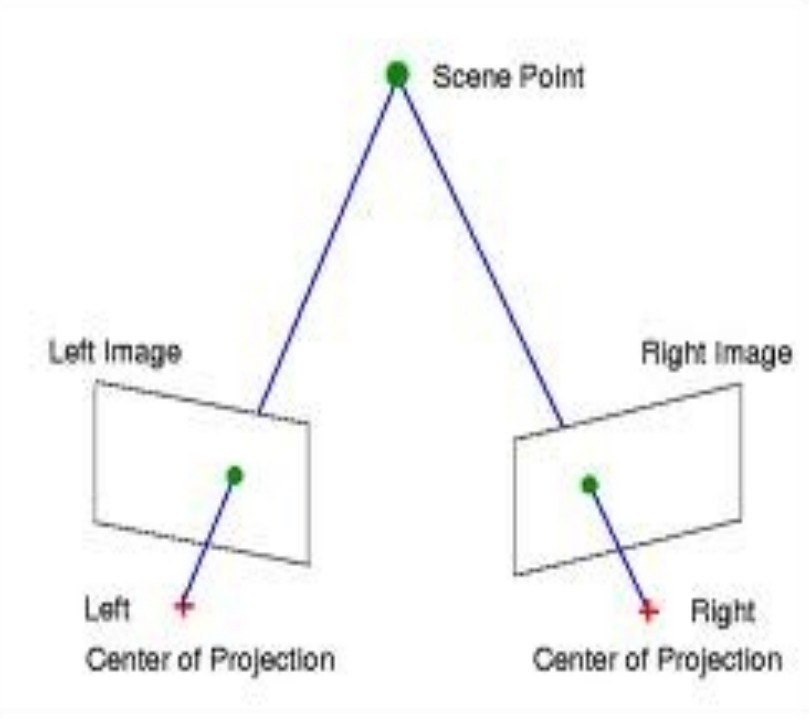
\includegraphics[width=5cm,height=3.3cm]{../Thesis_work/Latex_thesis_work/img_source/stereo_correspondence_abstract.png}}
\hspace{1cm}\subfloat[Stereo-correspondence]{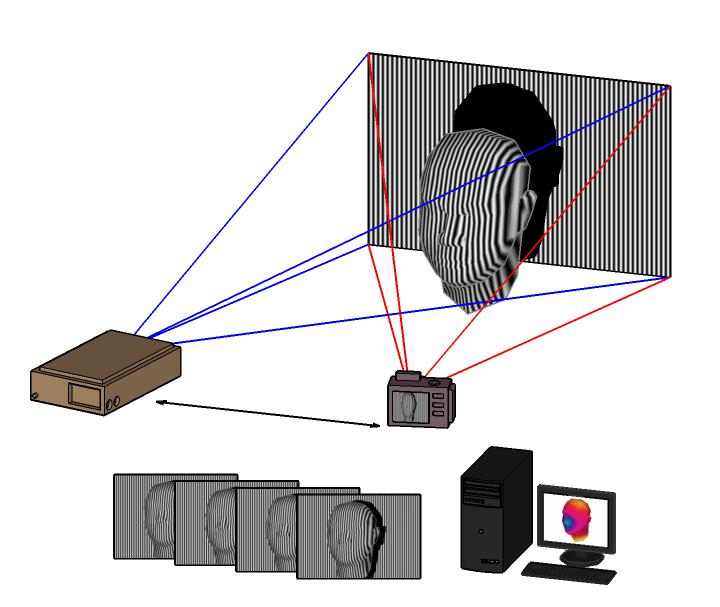
\includegraphics[width=5cm,height=3.3cm]{../Thesis_work/Latex_thesis_work/img_source/phase_shift.jpg}}
\end{figure}
\end{frame}
%%%%%%%%%%%%%%%%%%%%%%%%%%%%%%%%%%%%%%%%%%%%%%%%%%%%%%%%%%%%%%%%%%%%%%%%%%%%SLIDE ENDS%%%%%%%%%%%%%%%%%%%%%%%%%%%%%%%%%%%%%%%

%%%%%%%%%%%%%%%%%%%%%%%%%%%%%%%%%%%%%%%%%%%%%%%%%%%%%%%%%%%%%%%%%%%%%%%%%%%%%SLIDE starts%%%%%%%%%%%%%%%%%%%%%%%%%%%%%%%%%%%%%
\begin{frame}
\frametitle{Architecture of developed system}
\begin{figure}
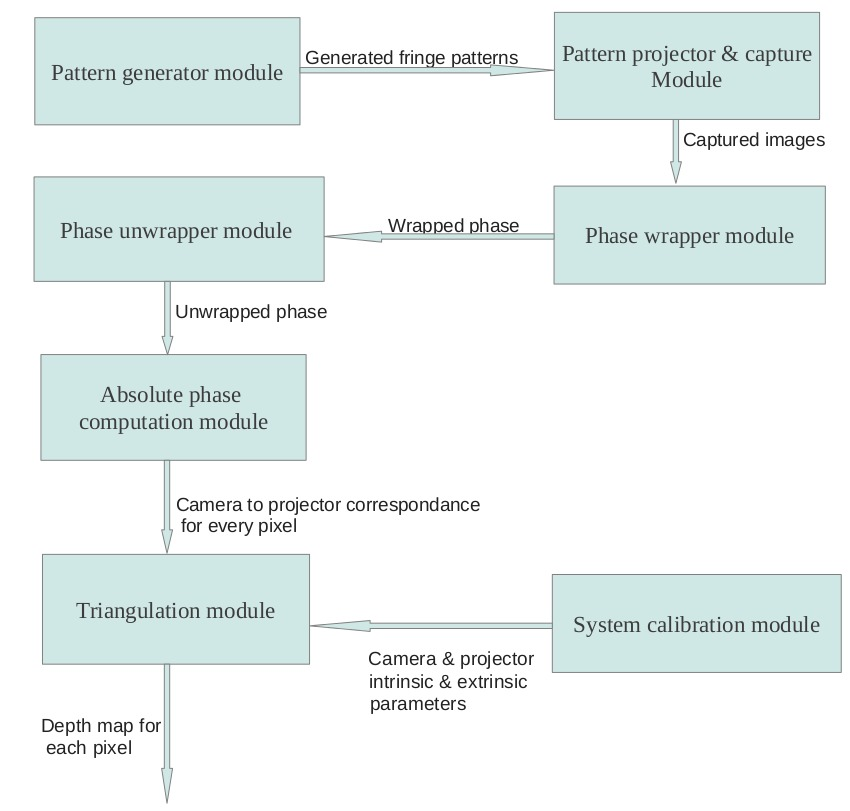
\includegraphics[width=8cm,height=7.5cm]{../Thesis_work/Latex_thesis_work/img_source/system_layout.png}
\caption{System architecture}
\end{figure}
\end{frame}
%%%%%%%%%%%%%%%%%%%%%%%%%%%%%%%%%%%%%%%%%%%%%%%%%%%%%%%%%%%%%%%%%%%%%%%%%%%%SLIDE ENDS%%%%%%%%%%%%%%%%%%%%%%%%%%%%%%%%%%%%%%%

%%%%%%%%%%%%%%%%%%%%%%%%%%%%%%%%%%%%%%%%%%%%%%%%%%%%%%%%%%%%%%%%%%%%%%%%%%%%%SLIDE starts%%%%%%%%%%%%%%%%%%%%%%%%%%%%%%%%%%%%%
\begin{frame}
\frametitle{System setup}
\begin{enumerate}
\item Sharp PG-F200X projector at 1024X768 resolution
\item Logitech Quickcam Sphere AF webcam at 1600X1200 resolution.
\item Developed system has been used and tested at Core i3-550 processor with 4GB RAM.
\end{enumerate}

\begin{figure}
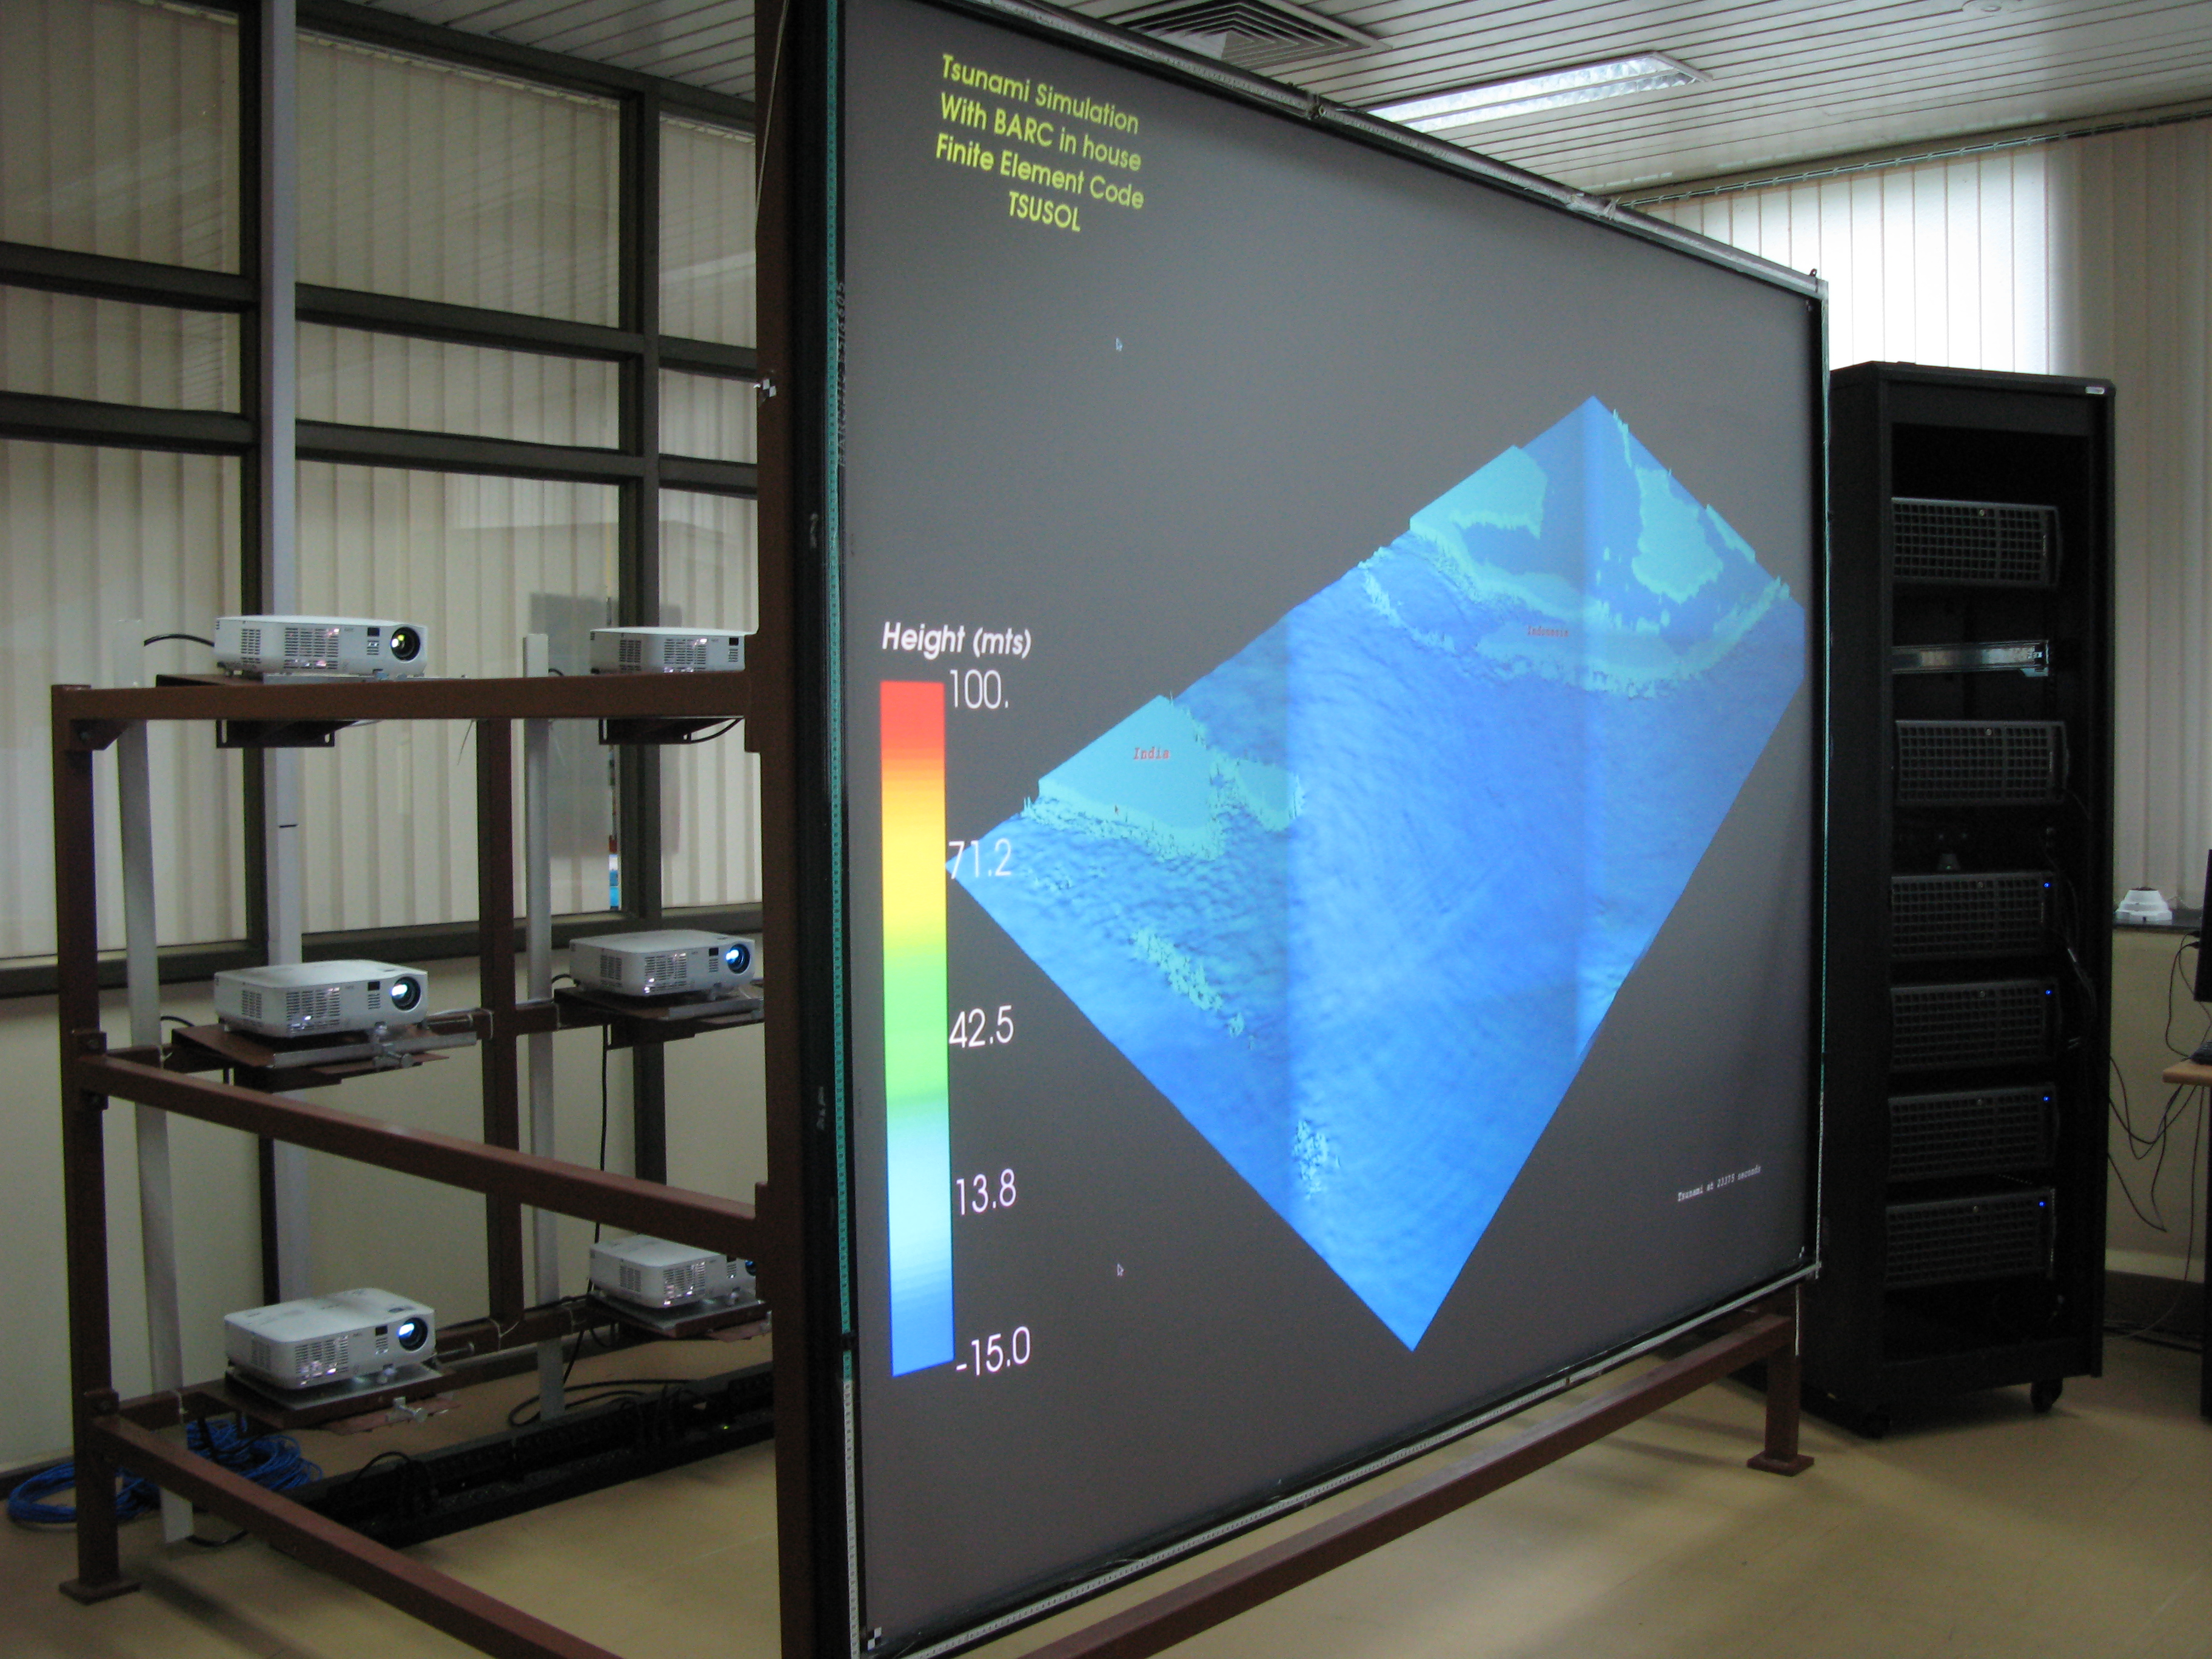
\includegraphics[width=5cm,height=5cm]{../Thesis_work/Latex_thesis_work/img_source/system_setup.png}
\end{figure}
\end{frame}
%%%%%%%%%%%%%%%%%%%%%%%%%%%%%%%%%%%%%%%%%%%%%%%%%%%%%%%%%%%%%%%%%%%%%%%%%%%%SLIDE ENDS%%%%%%%%%%%%%%%%%%%%%%%%%%%%%%%%%%%%%%%


%%%%%%%%%%%%%%%%%%%%%%%%%%%%%%%%%%%%%%%%%%%%%%%%%%%%%%%%%%%%%%%%%%%%%%%%%%%%%SLIDE starts%%%%%%%%%%%%%%%%%%%%%%%%%%%%%%%%%%%%%
\begin{frame}
\frametitle{Pattern generator module}
Vertical phase shifted patterns are defined by:\newline
\begin{equation}
\begin{aligned}
& P_1^v=A_v+B_v*cos(\theta_v-\alpha) \\
& P_2^v=A_v+B_v*cos(\theta_v) \\
& P_3^v=A_v+B_v*cos(\theta_v+\alpha) \\
\end{aligned}
\end{equation}
where $\theta_v=2\pi\frac{x}{fringe\ width}$

\begin{figure}[ht]
%\def\tabularxcolumn#1{m{#1}}
\begin{tabularx}{\linewidth}{@{}cXX@{}}
\begin{tabular}{c c c}
\hspace{1.5cm}\subfloat[]{
\includegraphics[width=3cm,height=3cm]{../Thesis_work/Latex_thesis_work/img_source/phase_ver_1.png}} &
\subfloat[]{
\includegraphics[width=3cm,height=3cm]{../Thesis_work/Latex_thesis_work/img_source/phase_ver_2.png}} &
\subfloat[]{
\includegraphics[width=3cm,height=3cm]{../Thesis_work/Latex_thesis_work/img_source/phase_ver_3.png}} \\ 
\end{tabular}
\end{tabularx}
\caption{Vertical phase-shifted patterns}
\label{fig:vert_phase_pattern}
\end{figure}
\end{frame}
%%%%%%%%%%%%%%%%%%%%%%%%%%%%%%%%%%%%%%%%%%%%%%%%%%%%%%%%%%%%%%%%%%%%%%%%%%%%SLIDE ENDS%%%%%%%%%%%%%%%%%%%%%%%%%%%%%%%%%%%%%%%


%%%%%%%%%%%%%%%%%%%%%%%%%%%%%%%%%%%%%%%%%%%%%%%%%%%%%%%%%%%%%%%%%%%%%%%%%%%%%SLIDE starts%%%%%%%%%%%%%%%%%%%%%%%%%%%%%%%%%%%%%
\begin{frame}
Horizontal phase-shifted patterns are defined by:\newline
\begin{equation}
\begin{aligned}
& P_1^h=A_h+B_h*cos(\theta_h-\alpha) \\
& P_2^h=A_h+B_h*cos(\theta_h) \\
& P_3^h=A_h+B_h*cos(\theta_h+\alpha) \\
\end{aligned}
\end{equation}
where $\theta_h=2\pi\frac{y}{fringe\ width}$

\begin{figure}[ht]
%\def\tabularxcolumn#1{m{#1}}
\begin{tabularx}{\linewidth}{@{}cXX@{}}
\begin{tabular}{c c c}
\hspace{1.5cm}\subfloat[]{
\includegraphics[width=3cm,height=3cm]{../Thesis_work/Latex_thesis_work/img_source/phase_hor_1.png}} &
\subfloat[]{
\includegraphics[width=3cm,height=3cm]{../Thesis_work/Latex_thesis_work/img_source/phase_hor_2.png}} &
\subfloat[]{
\includegraphics[width=3cm,height=3cm]{../Thesis_work/Latex_thesis_work/img_source/phase_hor_3.png}} \\ 
\end{tabular}
\end{tabularx}
\caption{Horizontal phase-shifted patterns}
\label{fig:horz_phase_pattern}
\end{figure}
\end{frame}
%%%%%%%%%%%%%%%%%%%%%%%%%%%%%%%%%%%%%%%%%%%%%%%%%%%%%%%%%%%%%%%%%%%%%%%%%%%%SLIDE ENDS%%%%%%%%%%%%%%%%%%%%%%%%%%%%%%%%%%%%%%%



%%%%%%%%%%%%%%%%%%%%%%%%%%%%%%%%%%%%%%%%%%%%%%%%%%%%%%%%%%%%%%%%%%%%%%%%%%%%SLIDE starts%%%%%%%%%%%%%%%%%%%%%%%%%%%%%%%%%%%%%%%
\begin{frame}
Vertical binary coded patterns are defined by:\newline
\begin{equation}
N_{v}^{codes}=\frac{W_{projector}}{w_{fringe}} 
\end{equation}
\begin{equation}
N_{v}^{patterns}=\log_2(N_v^{codes})
\end{equation}
\begin{equation}
Intensity_{(i,j)}=\lfloor i/{(w_{fringe}*2^{pattern\ number})} \rfloor
\end{equation}
\begin{figure}[ht]
\begin{tabularx}{\linewidth}{@{}cXX@{}}
\begin{tabular}{c c c}
\hspace{1.5cm}\subfloat[]{
\includegraphics[width=3cm,height=3cm]{../Thesis_work/Latex_thesis_work/img_source/binary_ver_1.png}} &
\subfloat[]{
\includegraphics[width=3cm,height=3cm]{../Thesis_work/Latex_thesis_work/img_source/binary_ver_2.png}} &
\subfloat[]{
\includegraphics[width=3cm,height=3cm]{../Thesis_work/Latex_thesis_work/img_source/binary_ver_3.png}} \\
\end{tabular}
\end{tabularx}
\caption{Vertical phase shifted patterns}
\end{figure}

\end{frame}
%%%%%%%%%%%%%%%%%%%%%%%%%%%%%%%%%%%%%%%%%%%%%%%%%%%%%%%%%%%%%%%%%%%%%%%%%%%%SLIDE ENDS%%%%%%%%%%%%%%%%%%%%%%%%%%%%%%%%%%%%%%%



%%%%%%%%%%%%%%%%%%%%%%%%%%%%%%%%%%%%%%%%%%%%%%%%%%%%%%%%%%%%%%%%%%%%%%%%%%%%%SLIDE starts%%%%%%%%%%%%%%%%%%%%%%%%%%%%%%%%%%%%%
\begin{frame}
Horizontal binary coded patterns are defined by:\newline
\begin{equation}
N_h^{codes}=\frac{H_{projector}}{w_{fringe}} 
\end{equation}
\begin{equation}
N_{h}^{patterns}=\log_2(N_h^{codes})
\end{equation}

\begin{equation}
Intensity_{(i,j)}=\lfloor j/{(w_{fringe}*2^{pattern\ number})} \rfloor
\end{equation}

\begin{figure}[ht]
\begin{tabularx}{\linewidth}{@{}cXX@{}}
\begin{tabular}{c c c}
\hspace{1.5cm}\subfloat[]{
\includegraphics[width=3cm,height=3cm]{../Thesis_work/Latex_thesis_work/img_source/binary_hor_1.png}} &
\subfloat[]{
\includegraphics[width=3cm,height=3cm]{../Thesis_work/Latex_thesis_work/img_source/binary_hor_2.png}} &
\subfloat[]{
\includegraphics[width=3cm,height=3cm]{../Thesis_work/Latex_thesis_work/img_source/binary_hor_3.png}} \\
\end{tabular}
\end{tabularx}
\caption{Horizontal binary coded patterns}
\end{figure}
\end{frame}
%%%%%%%%%%%%%%%%%%%%%%%%%%%%%%%%%%%%%%%%%%%%%%%%%%%%%%%%%%%%%%%%%%%%%%%%%%%%SLIDE ENDS%%%%%%%%%%%%%%%%%%%%%%%%%%%%%%%%%%%%%%%

%%%%%%%%%%%%%%%%%%%%%%%%%%%%%%%%%%%%%%%%%%%%%%%%%%%%%%%%%%%%%%%%%%%%%%%%%%%%%SLIDE starts%%%%%%%%%%%%%%%%%%%%%%%%%%%%%%%%%%%%%
\begin{frame}
\frametitle{Pattern projection and capture module}
\begin{figure}
\begin{tabularx}{\linewidth}{@{}cXX@{}}
\begin{tabular}{c c c}
\hspace{1cm}\subfloat[]{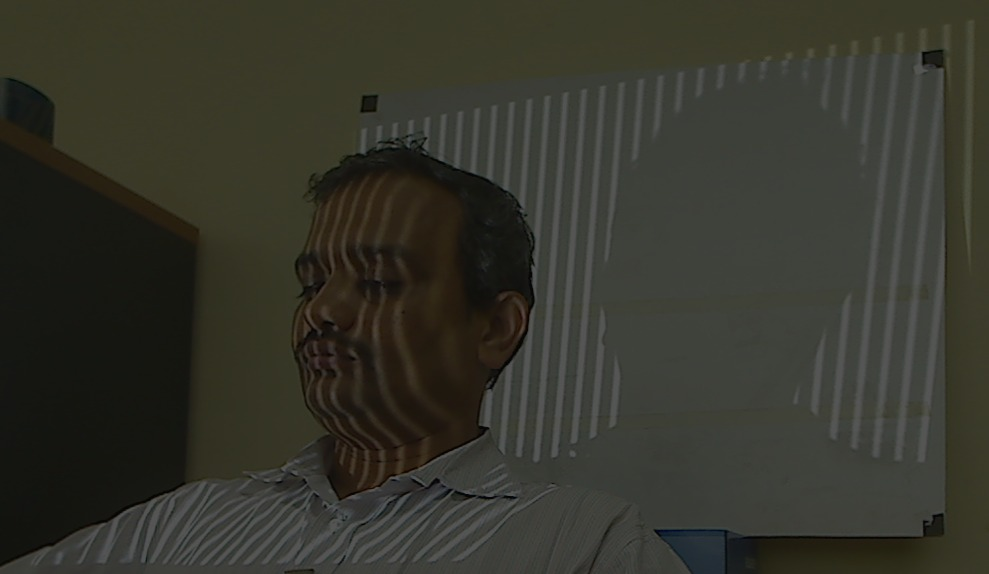
\includegraphics[width=3cm,height=3cm]{../Thesis_work/Latex_thesis_work/img_source/cap_fringe_1.png}} &
\subfloat[]{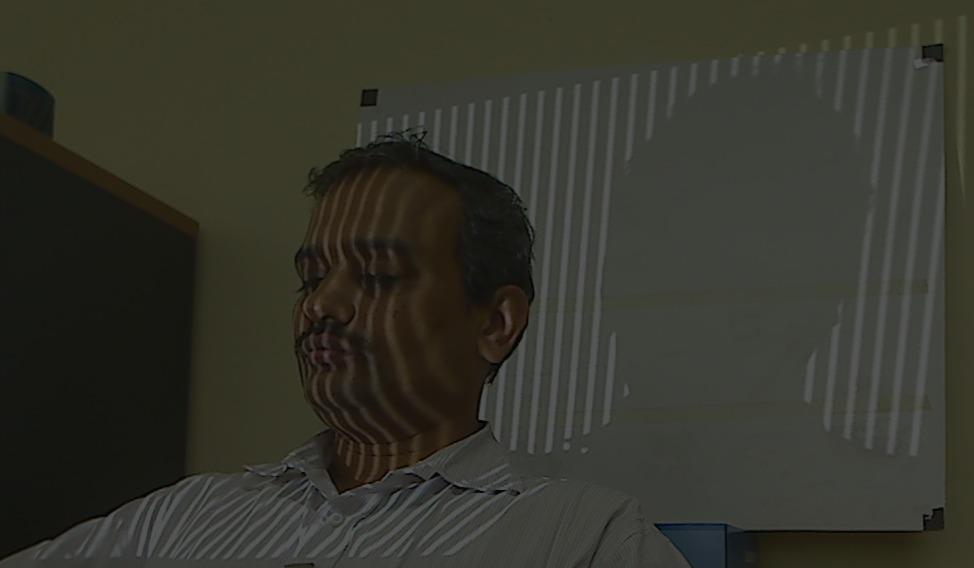
\includegraphics[width=3cm,height=3cm]{../Thesis_work/Latex_thesis_work/img_source/cap_fringe_2.png}} &
\subfloat[]{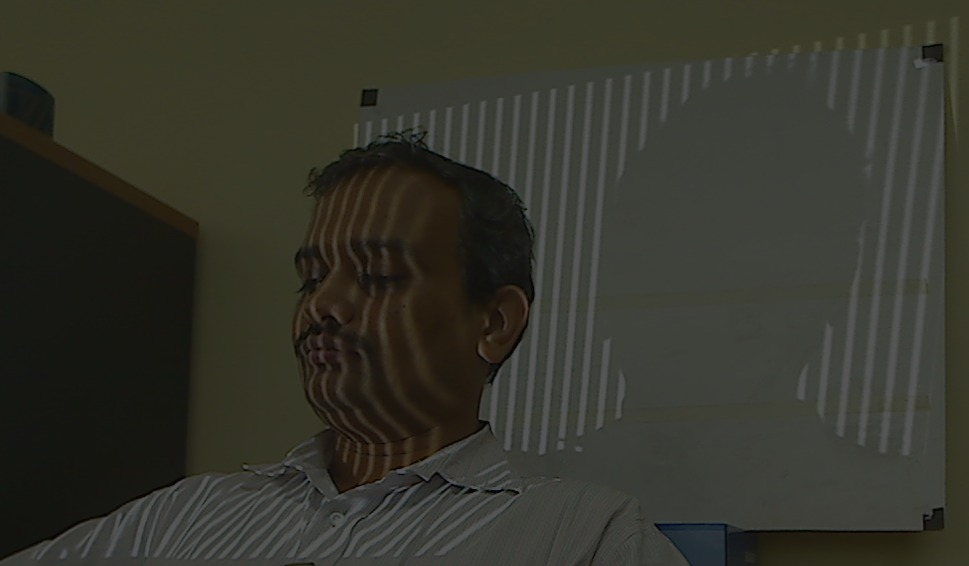
\includegraphics[width=3cm,height=3cm]{../Thesis_work/Latex_thesis_work/img_source/cap_fringe_3.png}} \\
\hspace{1cm}\subfloat[]{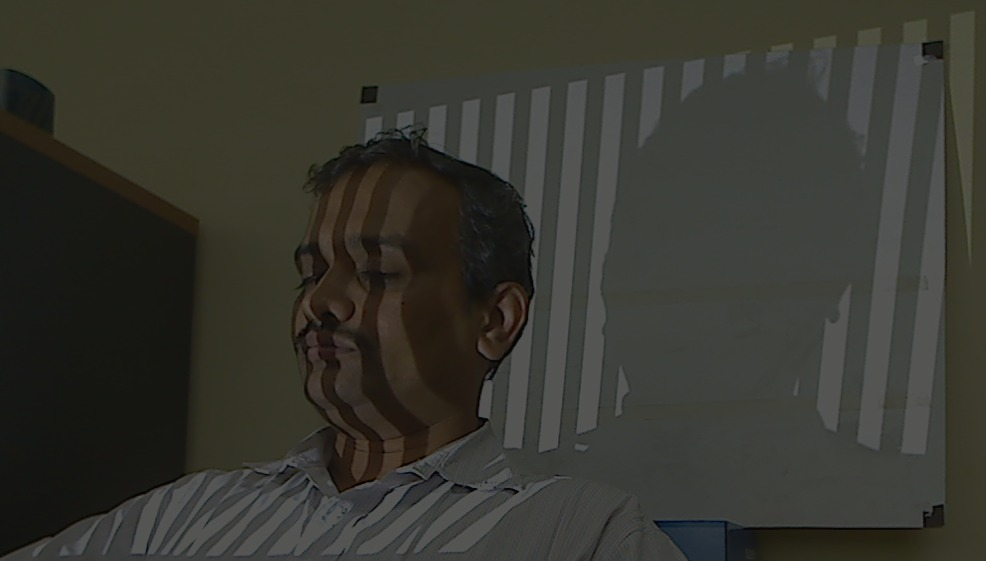
\includegraphics[width=3cm,height=3cm]{../Thesis_work/Latex_thesis_work/img_source/cap_fringe_4.png}} &
\subfloat[]{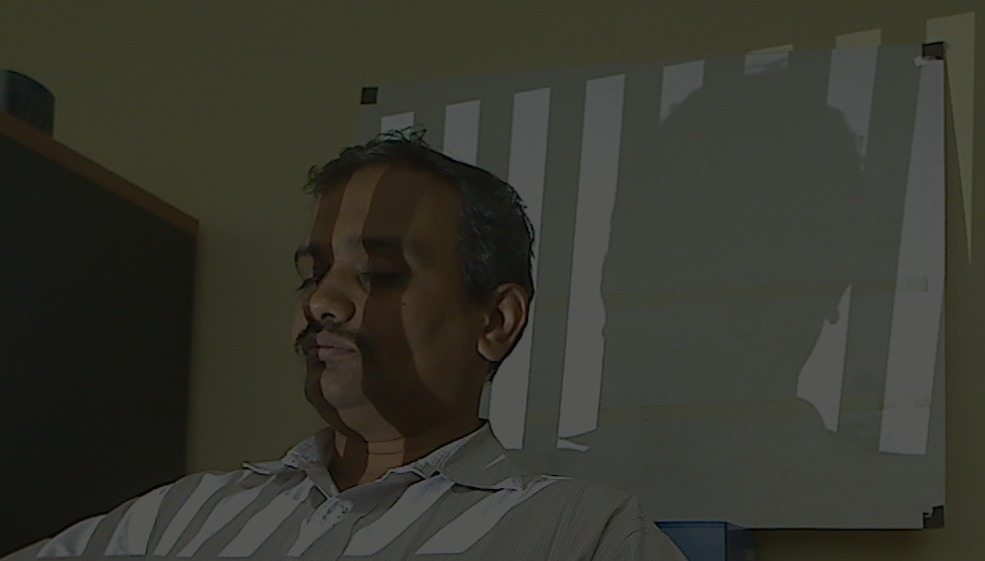
\includegraphics[width=3cm,height=3cm]{../Thesis_work/Latex_thesis_work/img_source/cap_fringe_5.png}} &
\subfloat[]{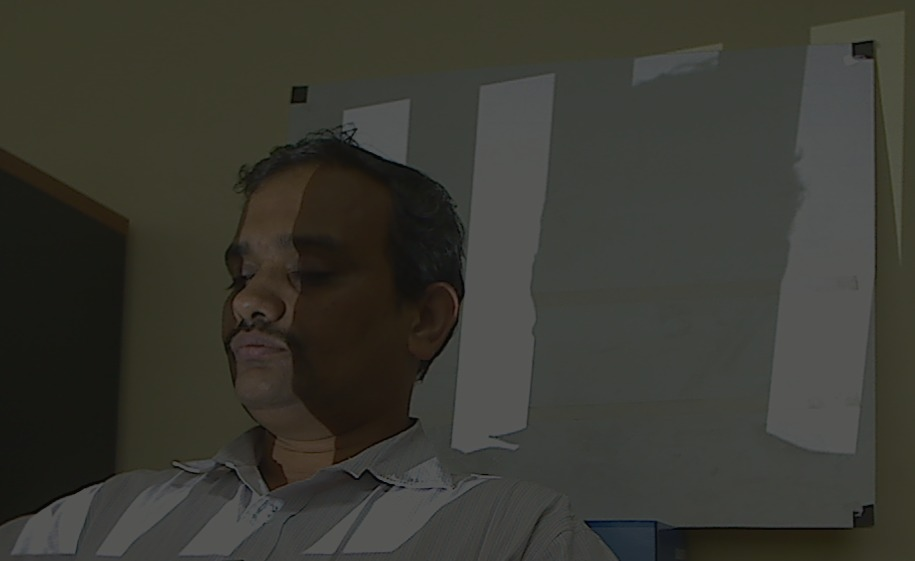
\includegraphics[width=3cm,height=3cm]{../Thesis_work/Latex_thesis_work/img_source/cap_fringe_6.png}} \\
\end{tabular}
\end{tabularx}
\caption{Captured vertical phase-shifted and binary coded patterns}
\end{figure}
\end{frame}
%%%%%%%%%%%%%%%%%%%%%%%%%%%%%%%%%%%%%%%%%%%%%%%%%%%%%%%%%%%%%%%%%%%%%%%%%%%%SLIDE ENDS%%%%%%%%%%%%%%%%%%%%%%%%%%%%%%%%%%%%%%%

%%%%%%%%%%%%%%%%%%%%%%%%%%%%%%%%%%%%%%%%%%%%%%%%%%%%%%%%%%%%%%%%%%%%%%%%%%%%%SLIDE starts%%%%%%%%%%%%%%%%%%%%%%%%%%%%%%%%%%%%%
\begin{frame}
\begin{figure}
\begin{tabularx}{\linewidth}{@{}cXX@{}}
\begin{tabular}{c c c}
\hspace{1cm}\subfloat[]{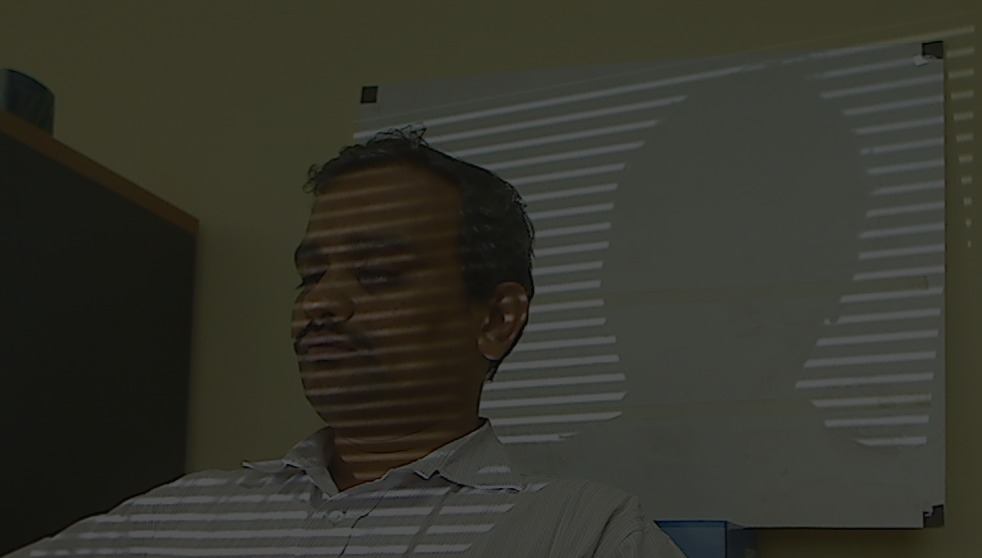
\includegraphics[width=3cm,height=3cm]{../Thesis_work/Latex_thesis_work/img_source/cap_binary_1.png}} &
\subfloat[]{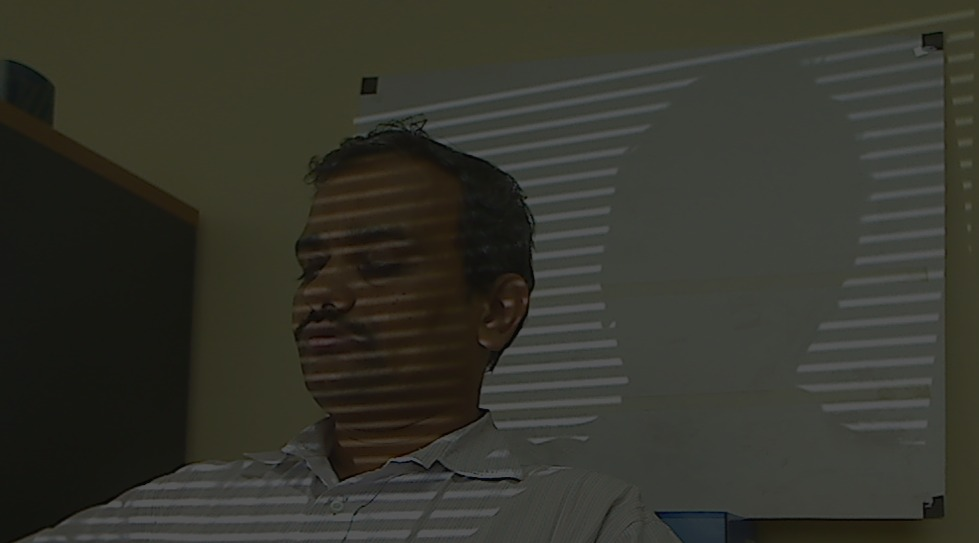
\includegraphics[width=3cm,height=3cm]{../Thesis_work/Latex_thesis_work/img_source/cap_binary_2.png}} &
\subfloat[]{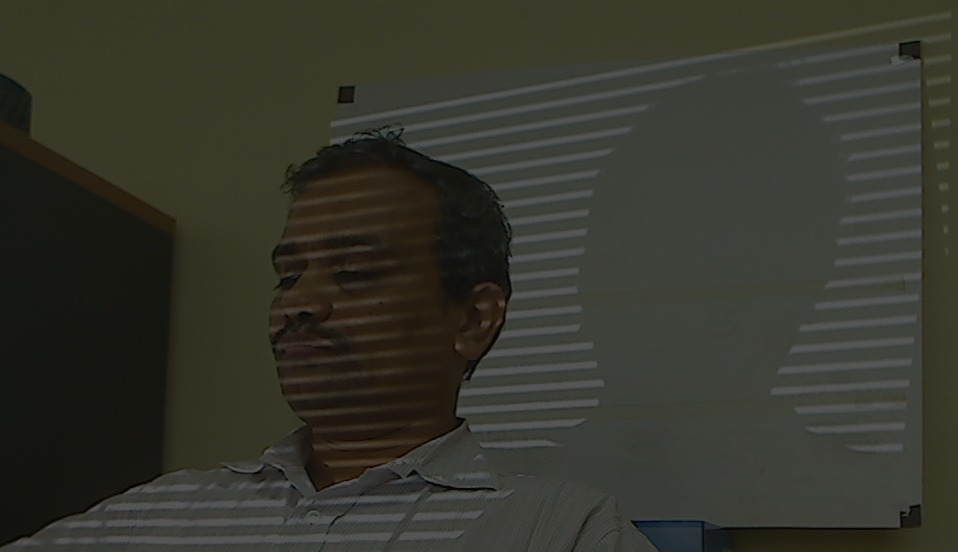
\includegraphics[width=3cm,height=3cm]{../Thesis_work/Latex_thesis_work/img_source/cap_binary_3.png}} \\
\hspace{1cm}\subfloat[]{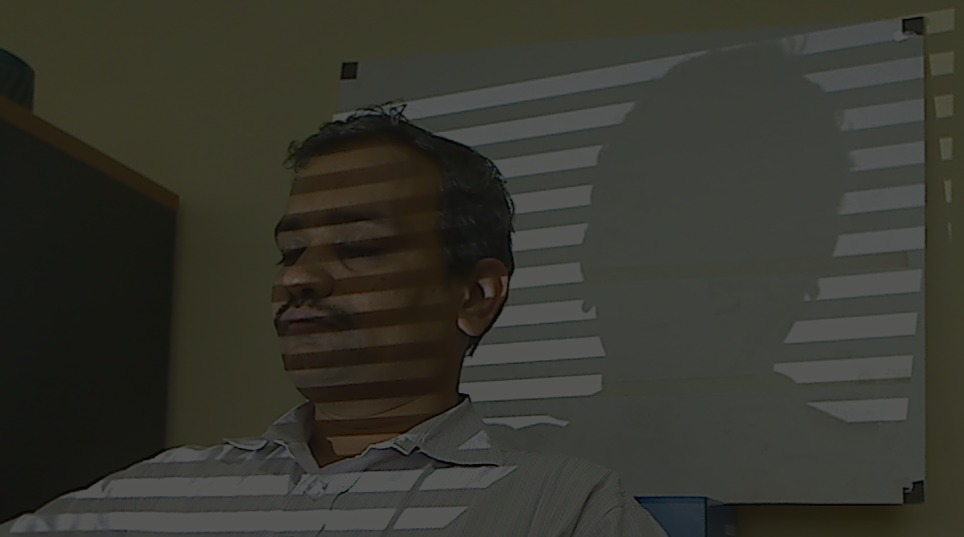
\includegraphics[width=3cm,height=3cm]{../Thesis_work/Latex_thesis_work/img_source/cap_binary_4.png}} &
\subfloat[]{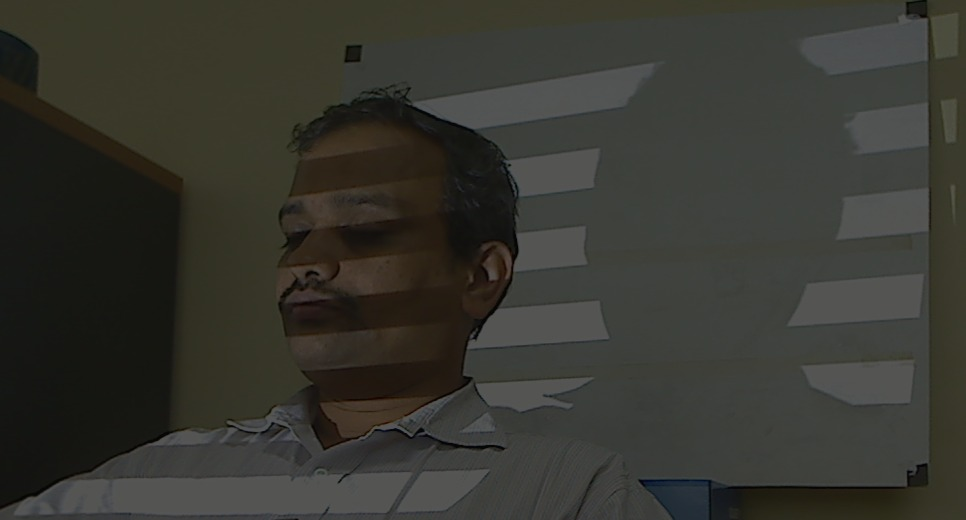
\includegraphics[width=3cm,height=3cm]{../Thesis_work/Latex_thesis_work/img_source/cap_binary_5.png}} &
\subfloat[]{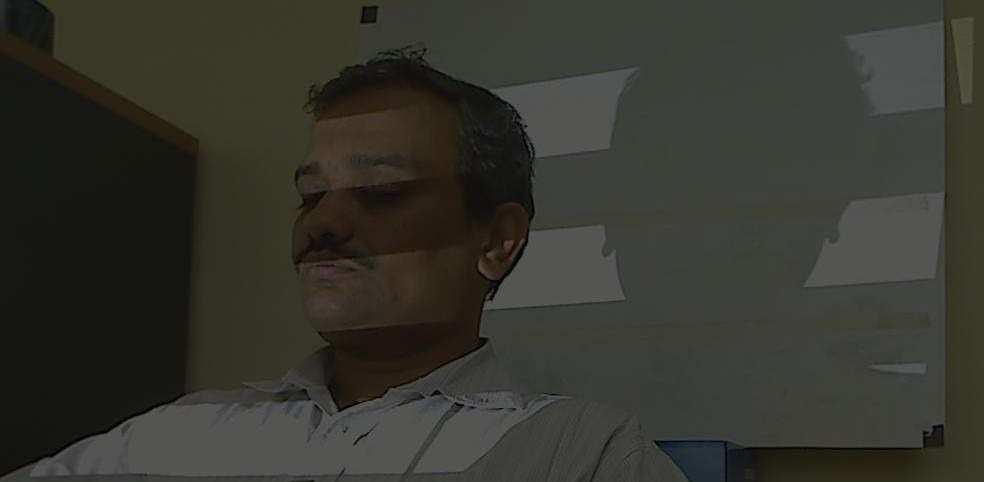
\includegraphics[width=3cm,height=3cm]{../Thesis_work/Latex_thesis_work/img_source/cap_binary_6.png}}
\end{tabular}
\end{tabularx}
\caption{Captured horizontal phase-shifted and binary coded patterns}
\end{figure}
\end{frame}
%%%%%%%%%%%%%%%%%%%%%%%%%%%%%%%%%%%%%%%%%%%%%%%%%%%%%%%%%%%%%%%%%%%%%%%%%%%%SLIDE ENDS%%%%%%%%%%%%%%%%%%%%%%%%%%%%%%%%%%%%%%%


%%%%%%%%%%%%%%%%%%%%%%%%%%%%%%%%%%%%%%%%%%%%%%%%%%%%%%%%%%%%%%%%%%%%%%%%%%%%%SLIDE starts%%%%%%%%%%%%%%%%%%%%%%%%%%%%%%%%%%%%%
\begin{frame}
\frametitle{Phase wrapping module}
Assumed illumination model for 3 phase shifted pattern approach:
\begin{equation}
\begin{aligned}
& I_1^{v/h}=I_{dc}^{v/h}+I_{mod}^{v/h}*cos(\theta_{v/h}-\alpha) \\
& I_2^{v/h}=I_{dc}^{v/h}+I_{mod}^{v/h}*cos(\theta_{v/h}) \\
& I_3^{v/h}=I_{dc}^{v/h}+I_{mod}^{v/h}*cos(\theta_{v/h}+\alpha)
\end{aligned}
\end{equation}
Hence,
\begin{equation}
\begin{aligned}
& \theta_v=tan^{-1}\bigg[\frac{\sqrt[2]{3}(I_1^v-I_3^v)}{2I_2^v-I_1^v-I_3^v}\bigg],-\pi\leq\theta_v\leq\pi,
& \theta_h=tan^{-1}\bigg[\frac{\sqrt[2]{3}(I_1^h-I_3^h)}{2I_2^h-I_1^h-I_3^h}\bigg],-\pi\leq\theta_h\leq\pi 
\end{aligned}
\end{equation}
\begin{figure}[ht]
%\def\tabularxcolumn#1{m{#1}}
\begin{tabularx}{\linewidth}{@{}cXX@{}}
\begin{tabular}{l r}
\hspace{3cm}\subfloat[Vertical wrapped phase]{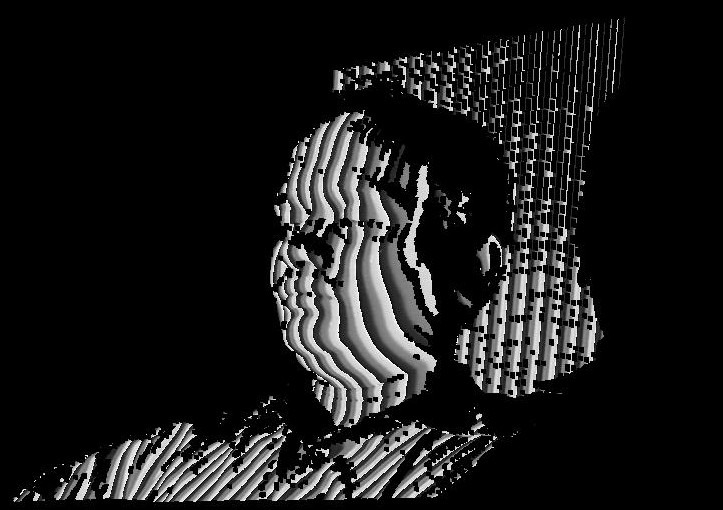
\includegraphics[width=3cm,height=3cm]{../Thesis_work/Latex_thesis_work/img_source/wrapped_ver.png}} &
\subfloat[Horizontal wrapped phase]{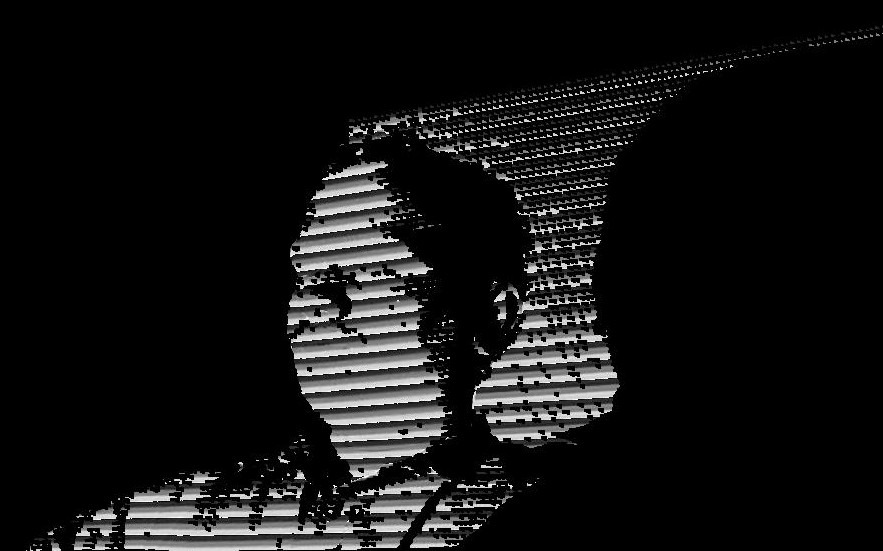
\includegraphics[width=3cm,height=3cm]{../Thesis_work/Latex_thesis_work/img_source/wrapped_hor.png}}\\
\end{tabular}
\end{tabularx}
\caption{Computed wrapped phase}
\label{fig:wrapped_phase}
\end{figure}
\end{frame}
%%%%%%%%%%%%%%%%%%%%%%%%%%%%%%%%%%%%%%%%%%%%%%%%%%%%%%%%%%%%%%%%%%%%%%%%%%%%SLIDE ENDS%%%%%%%%%%%%%%%%%%%%%%%%%%%%%%%%%%%%%%%

%%%%%%%%%%%%%%%%%%%%%%%%%%%%%%%%%%%%%%%%%%%%%%%%%%%%%%%%%%%%%%%%%%%%%%%%%%%%%SLIDE starts%%%%%%%%%%%%%%%%%%%%%%%%%%%%%%%%%%%%%
\begin{frame}
\frametitle{Phase unwrapping module}
Unwrapped phase $(\psi_v,\psi_h)$ maps $(\theta_v,\theta_h)$ to its correct $2\pi$ multiple:
\begin{equation}
\begin{aligned}
& \psi_v=\theta_v+2\pi*C_v \\
& \psi_h=\theta_h+2\pi*C_h
\end{aligned}
\end{equation}
where,\newline
\indent 
$C_v(x,y)$: Decoded vertical binary code(or \textit{vertical period number}) at any pixel (x,y).\newline
$C_h(x,y)$: Decoded horizontal binary code(or \textit{horizontal period number}) at any pixel (x,y).
\begin{figure}[ht]
%\def\tabularxcolumn#1{m{#1}}
\begin{tabularx}{\linewidth}{@{}cXX@{}}
\begin{tabular}{l r}
\hspace{3cm}\subfloat[Vertical unwrapped phase]{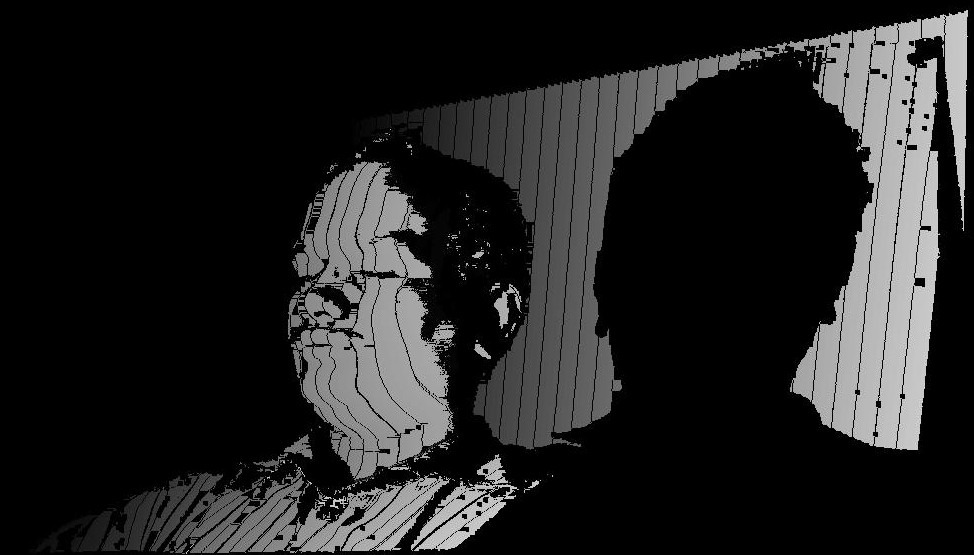
\includegraphics[width=3cm,height=3cm]{../Thesis_work/Latex_thesis_work/img_source/unwrapped_ver.png}} &
\subfloat[Horizontal unwrapped phase]{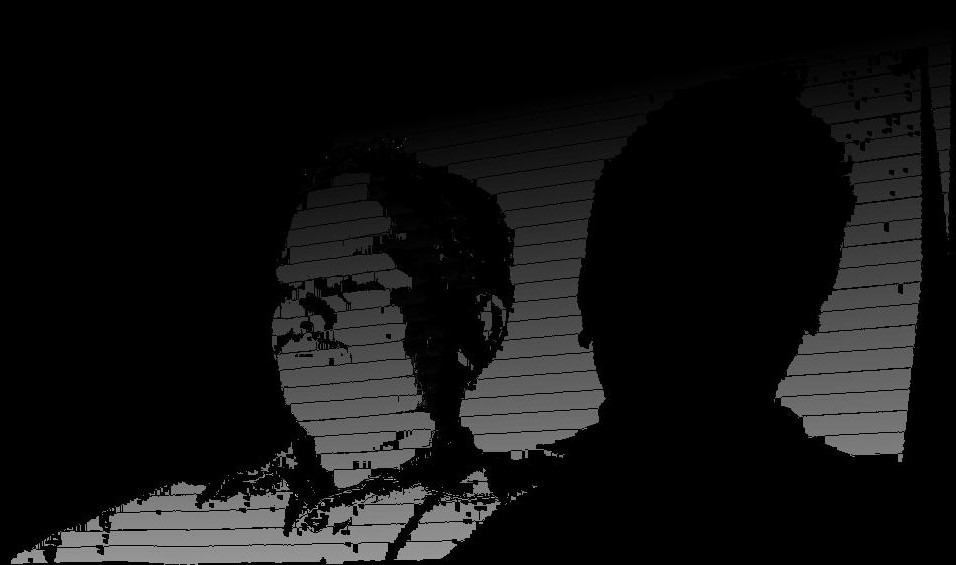
\includegraphics[width=3cm,height=3cm]{../Thesis_work/Latex_thesis_work/img_source/unwrapped_hor.png}}\\
\end{tabular}
\end{tabularx}
\caption{Computed unwrapped phase}
\label{fig:unwrapped_phase}
\end{figure}
\end{frame}
%%%%%%%%%%%%%%%%%%%%%%%%%%%%%%%%%%%%%%%%%%%%%%%%%%%%%%%%%%%%%%%%%%%%%%%%%%%%SLIDE ENDS%%%%%%%%%%%%%%%%%%%%%%%%%%%%%%%%%%%%%%%

%%%%%%%%%%%%%%%%%%%%%%%%%%%%%%%%%%%%%%%%%%%%%%%%%%%%%%%%%%%%%%%%%%%%%%%%%%%%%SLIDE starts%%%%%%%%%%%%%%%%%%%%%%%%%%%%%%%%%%%%%
\begin{frame}
\frametitle{Absolute phase computation module}
Computing projector coordinates $(X_p,Y_p)$ corresponding to a camera coordinates $(X_c,Y_c)$
\begin{equation}
\begin{aligned}
& X_p=\lfloor w_{fringe}*\big(\frac{\psi_v}{2\pi}\big) \rfloor  ,
%2\pi*\bigg\lfloor\frac{\psi_v(X_c,Y_c)}{2\pi}\bigg\rfloor+2\pi*\bigg(\frac{\psi_v(X_c,Y_c)}{2\pi}-\bigg\lfloor\frac{\psi_v(X_c,Y_c)}{2\pi}\bigg\rfloor\bigg) \\
& Y_p=\lfloor w_{fringe}*\big(\frac{\psi_h}{2\pi}\big) \rfloor%2\pi*\bigg\lfloor\frac{\psi_h(X_c,Y_c)}{2\pi}\bigg\rfloor+2\pi*\bigg(\frac{\psi_h(X_c,Y_c)}{2\pi}-\bigg\lfloor\frac{\psi_h(X_c,Y_c)}{2\pi}\bigg\rfloor\bigg)
\end{aligned}
\end{equation}
\begin{figure}
%\def\tabularxcolumn#1{m{#1}}
\begin{tabularx}{\linewidth}{@{}cXX@{}}
\begin{tabular}{c c}
\hspace{2cm}
\subfloat[Camera image]{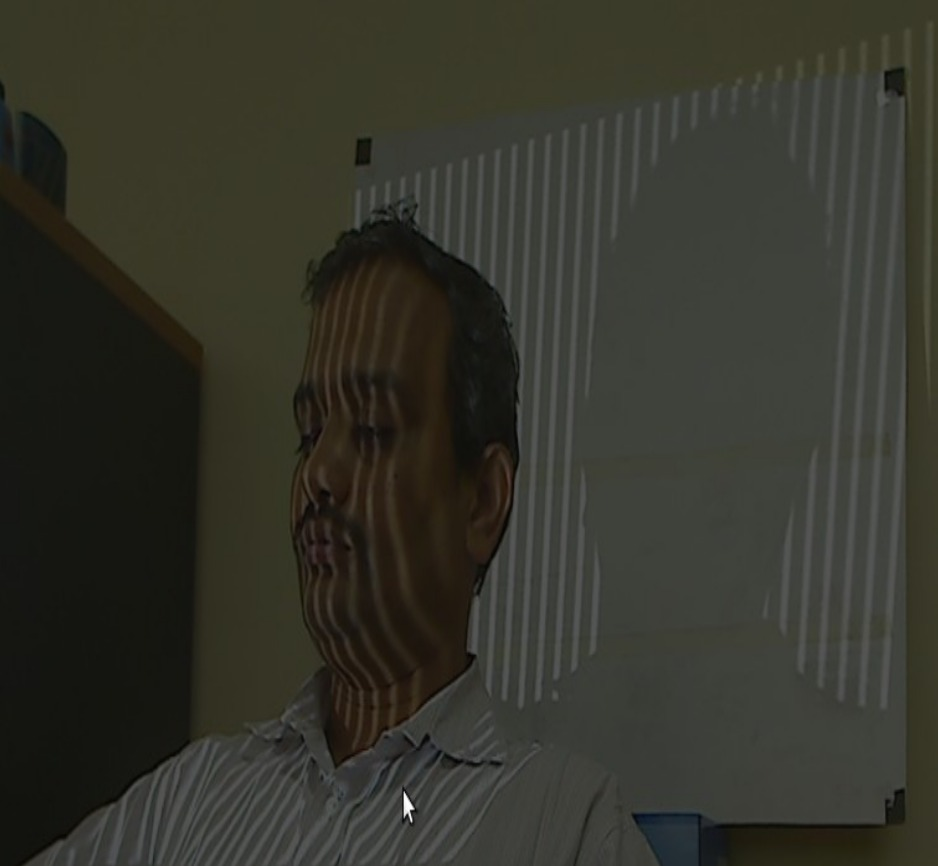
\includegraphics[width=3cm,height=3cm]{../Thesis_work/Latex_thesis_work/img_source/camera_image.png}} &
\subfloat[Projector image]{
\includegraphics[width=3cm,height=3cm]{../Thesis_work/Latex_thesis_work/img_source/projector_image.png}} 
\end{tabular}
\end{tabularx}
\caption{Stereo correspondence between camera and projector}
\label{fig:estimated_correspondence}
\end{figure}
\end{frame}
%%%%%%%%%%%%%%%%%%%%%%%%%%%%%%%%%%%%%%%%%%%%%%%%%%%%%%%%%%%%%%%%%%%%%%%%%%%%SLIDE ENDS%%%%%%%%%%%%%%%%%%%%%%%%%%%%%%%%%%%%%%%


%%%%%%%%%%%%%%%%%%%%%%%%%%%%%%%%%%%%%%%%%%%%%%%%%%%%%%%%%%%%%%%%%%%%%%%%%%%%%SLIDE starts%%%%%%%%%%%%%%%%%%%%%%%%%%%%%%%%%%%%%
\begin{frame}
\frametitle{System calibration module}
\textbf{Intrinsic parameters}\newline  
$f_x$: focal length of lens expressed in number of pixels along X - axis\newline  
$f_y$: focal length of lens expressed in number of pixels along Y - axis\newline  
$(c_x , c_y)$: Pixel coordinates of principal point\newline  
$(k_1, k_2, k_3)$: Radial distortion coefficients\newline  
$(p_1,p_2)$: Tangential distortion coefficients\newline  
\textbf{Extrinsic parameters}\newline  
$(r_x,r_y,r_z)$: Rotation vector between camera(or projector) \& world coordinate system\newline  
$(t_x,t_y,t_z)$: Translation vector between camera(or projector) \& world coordinate system 
\begin{figure}
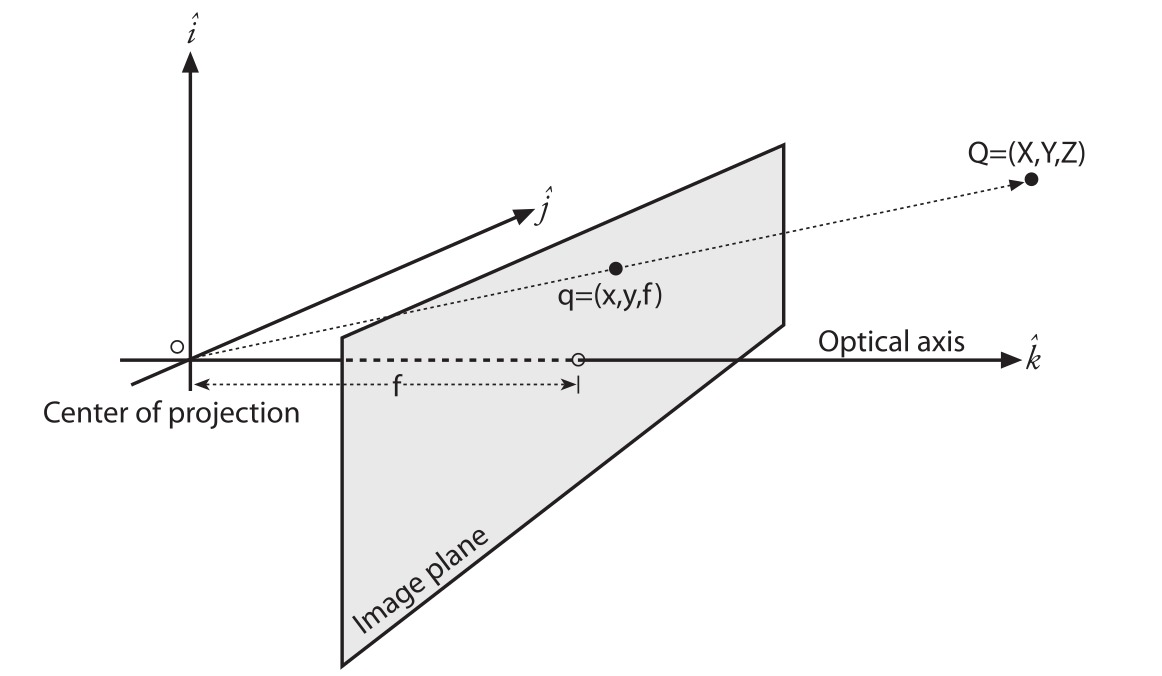
\includegraphics[width=7cm,height=4cm]{../Thesis_work/Latex_thesis_work/img_source/camera_model.png}
\caption{Pin-hole camera model}
\end{figure}
\end{frame}
%%%%%%%%%%%%%%%%%%%%%%%%%%%%%%%%%%%%%%%%%%%%%%%%%%%%%%%%%%%%%%%%%%%%%%%%%%%%SLIDE ENDS%%%%%%%%%%%%%%%%%%%%%%%%%%%%%%%%%%%%%%%
%%%%%%%%%%%%%%%%%%%%%%%%%%%%%%%%%%%%%%%%%%%%%%%%%%%%%%%%%%%%%%%%%%%%%%%%%%%%%SLIDE starts%%%%%%%%%%%%%%%%%%%%%%%%%%%%%%%%%%%%%
\begin{frame}
Mathematically,camera(or projector) model:
\begin{equation}
\begin{aligned}
& \begin{bmatrix}
U_e^i \\
V_e^i
\end{bmatrix} 
=A_c[R|T]\begin{bmatrix}
X_w^i \\
Y_w^i \\
Z_w^i
\end{bmatrix} \\
& \begin{bmatrix}
X_e^i \\
Y_e^i
\end{bmatrix}
=f(U_e^i,V_e^i)
\end{aligned}
\end{equation}

%Abstract description of intrinsic parameter calibration algorithm(OpenCV):
%\begin{enumerate}
%\item Computes the initial intrinsic parameters(assuming zero distortion coefficients).
%\item The initial camera pose is estimated as if the intrinsic parameters have been already known.
%\item Then the global \textit{Levenberg-Marquardt optimization algorithm} is run to minimize the \textit{reprojection error}.
%\end{enumerate}
OpenCV camera calibration algorithm is used which minimizes:\newline
\begin{equation}
\varepsilon=\sum_{i=1}^{N}\bigg[\sqrt[2]{(observed_x-projected_x)^2+(observed_y-projected_y)^2}\bigg]
\end{equation}
Extrinsic parameters that minimize reprojection error are considered as the \textit{optimal} pose(Rotation \& translation)  
parameters.\newline

\end{frame}
%%%%%%%%%%%%%%%%%%%%%%%%%%%%%%%%%%%%%%%%%%%%%%%%%%%%%%%%%%%%%%%%%%%%%%%%%%%%SLIDE ENDS%%%%%%%%%%%%%%%%%%%%%%%%%%%%%%%%%%%%%%%

%%%%%%%%%%%%%%%%%%%%%%%%%%%%%%%%%%%%%%%%%%%%%%%%%%%%%%%%%%%%%%%%%%%%%%%%%%%%%SLIDE starts%%%%%%%%%%%%%%%%%%%%%%%%%%%%%%%%%%%%%
\begin{frame}
\frametitle{Camera calibration}
\begin{figure}   
%\def\tabularxcolumn#1{m{#1}}  
\begin{tabularx}{\linewidth}{@{}cXX@{}}  
\begin{tabular}{c c c c}  
\hspace{-0.5cm}\subfloat[]{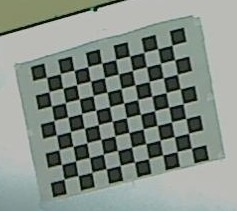
\includegraphics[width=3cm,height=3cm]{../Thesis_work/Latex_thesis_work/img_source/cam_1.png}} &  
\hspace{-0.3cm}\subfloat[]{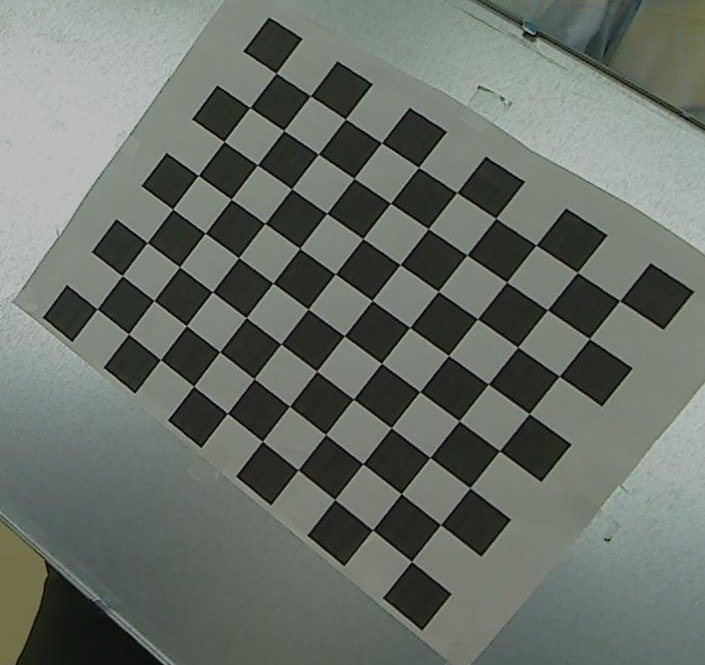
\includegraphics[width=3cm,height=3cm]{../Thesis_work/Latex_thesis_work/img_source/cam_2.png}} &  
\hspace{-0.3cm}\subfloat[]{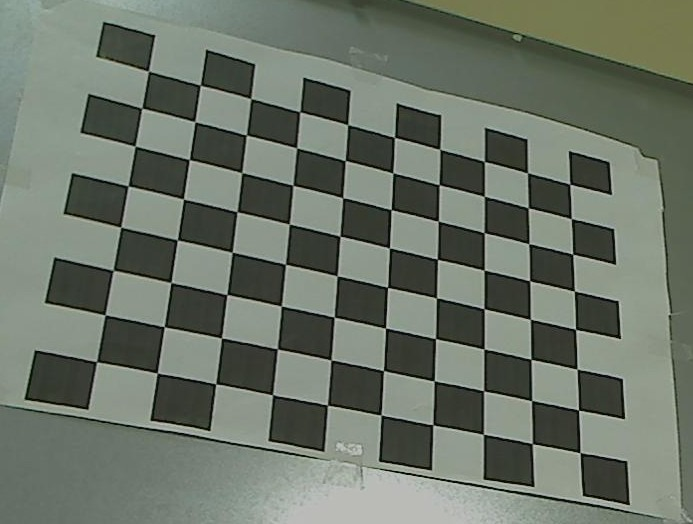
\includegraphics[width=3cm,height=3cm]{../Thesis_work/Latex_thesis_work/img_source/cam_3.png}} &  
\hspace{-0.3cm}\subfloat[]{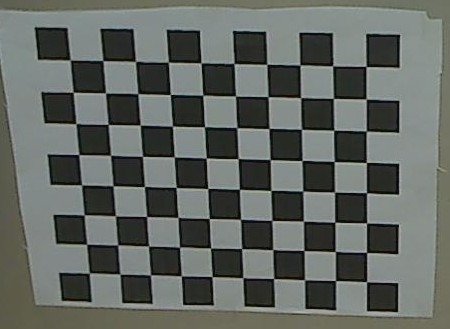
\includegraphics[width=3cm,height=3cm]{../Thesis_work/Latex_thesis_work/img_source/cam_4.png}}\\  
\end{tabular}  
\end{tabularx}  
\caption{Some views used for camera calibration}  
\label{fig:cam_calib_views}
\end{figure}  
\vspace{-0.5cm}
\begin{table}[ht]  
\centering  
\begin{tabular}{c l}  
\hline\noalign{\smallskip}  
Parameter & Estimated value \\  
\noalign{\smallskip}\hline\noalign{\smallskip}  
$f_x$ & 1362.152\\  
$f_y$ & 1372.189\\  
$c_x$ & 803.884\\  
$c_y$ & 590.066\\  
$k_1$ & 0.073\\  
$k_2$ & -0.143\\   
Reprojection error & 0.195 \\  
\noalign{\smallskip}\hline  
\end{tabular}  
\caption{Estimated Camera intrinsic model parameters}  
\end{table}  
\end{frame}
%%%%%%%%%%%%%%%%%%%%%%%%%%%%%%%%%%%%%%%%%%%%%%%%%%%%%%%%%%%%%%%%%%%%%%%%%%%%SLIDE ENDS%%%%%%%%%%%%%%%%%%%%%%%%%%%%%%%%%%%%%%%

%%%%%%%%%%%%%%%%%%%%%%%%%%%%%%%%%%%%%%%%%%%%%%%%%%%%%%%%%%%%%%%%%%%%%%%%%%%%%SLIDE starts%%%%%%%%%%%%%%%%%%%%%%%%%%%%%%%%%%%%%
\begin{frame}
SciLab script was developed to visualize calibration results for camera and projector calibration.
\begin{figure} 
\begin{tabularx}{\linewidth}{@{}cXX@{}}
\begin{tabular}{l r}
\subfloat[View along X-axis]{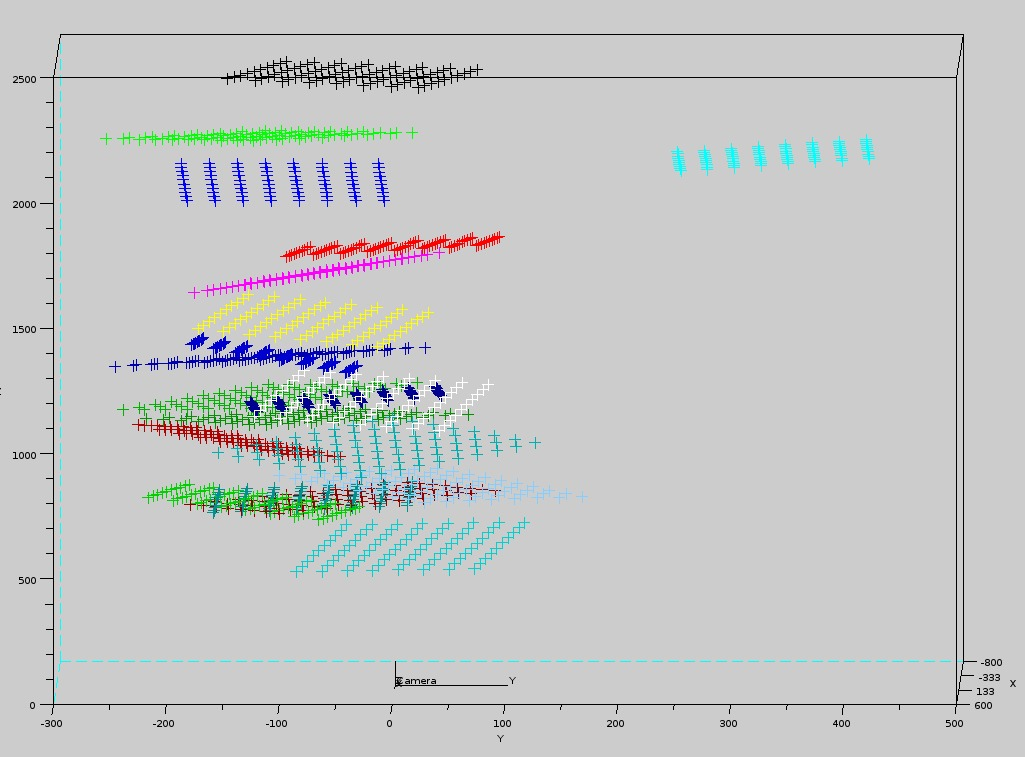
\includegraphics[width=6cm,height=6cm]{../Thesis_work/Latex_thesis_work/img_source/cam_calib_view.png}} &  
\hspace{-0.3cm}\subfloat[View along Y-axis]{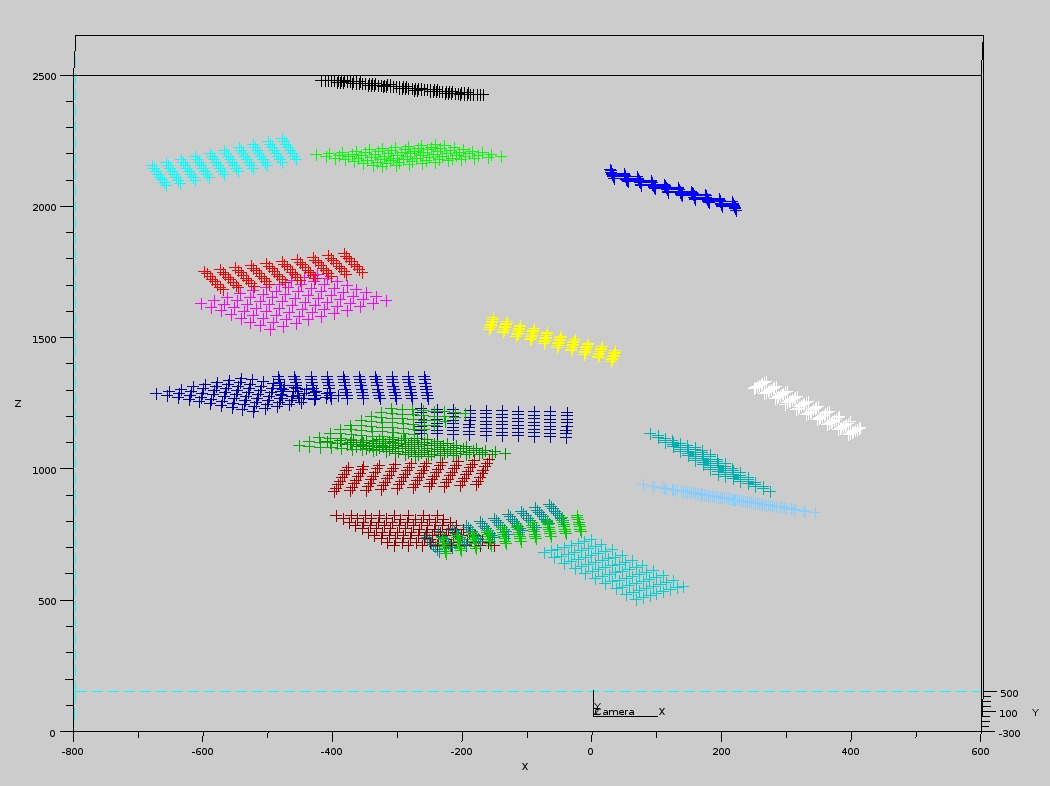
\includegraphics[width=6cm,height=6cm]{../Thesis_work/Latex_thesis_work/img_source/cam_calib_view2.png}} \\  
\end{tabular}
\end{tabularx} 
\caption{Visualization of camera calibration results} 
\end{figure}  
\end{frame}
%%%%%%%%%%%%%%%%%%%%%%%%%%%%%%%%%%%%%%%%%%%%%%%%%%%%%%%%%%%%%%%%%%%%%%%%%%%%SLIDE ENDS%%%%%%%%%%%%%%%%%%%%%%%%%%%%%%%%%%%%%%%

%%%%%%%%%%%%%%%%%%%%%%%%%%%%%%%%%%%%%%%%%%%%%%%%%%%%%%%%%%%%%%%%%%%%%%%%%%%%%SLIDE starts%%%%%%%%%%%%%%%%%%%%%%%%%%%%%%%%%%%%%
\begin{frame}
\frametitle{Projector calibration}
\begin{enumerate}
\item Projector assumed as \textit{inverse camera}.
\item Camera used as a feedback device which will provide the 3D coordinates for the 2D features projected by the projector.
\end{enumerate}
\begin{figure}[h!]  
%\def\tabularxcolumn#1{m{#1}}  
\begin{tabularx}{\linewidth}{@{}cXX@{}}  
\begin{tabular}{c c c c}   
\hspace{-0.3cm}\subfloat[]{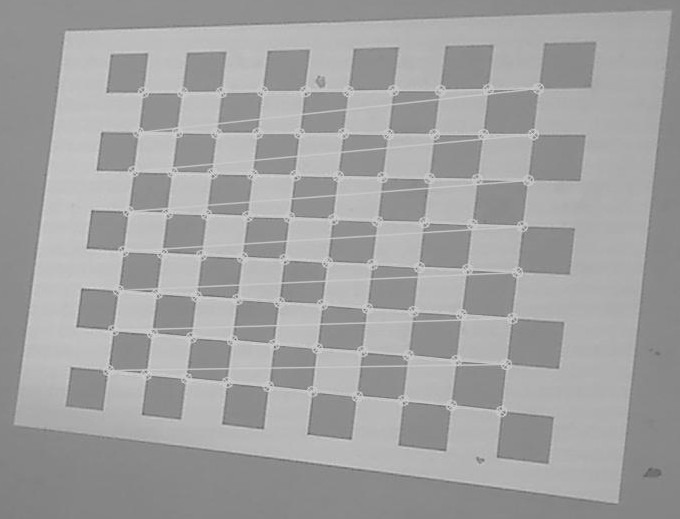
\includegraphics[width=3cm,height=3cm]{../Thesis_work/Latex_thesis_work/img_source/proj_view_1.png}} &  
\hspace{-0.3cm}\subfloat[]{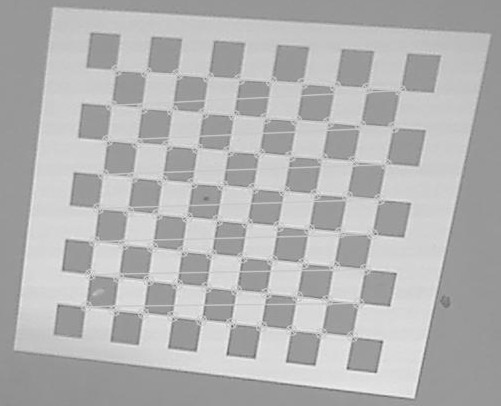
\includegraphics[width=3cm,height=3cm]{../Thesis_work/Latex_thesis_work/img_source/proj_view_2.png}} &  
\hspace{-0.3cm}\subfloat[]{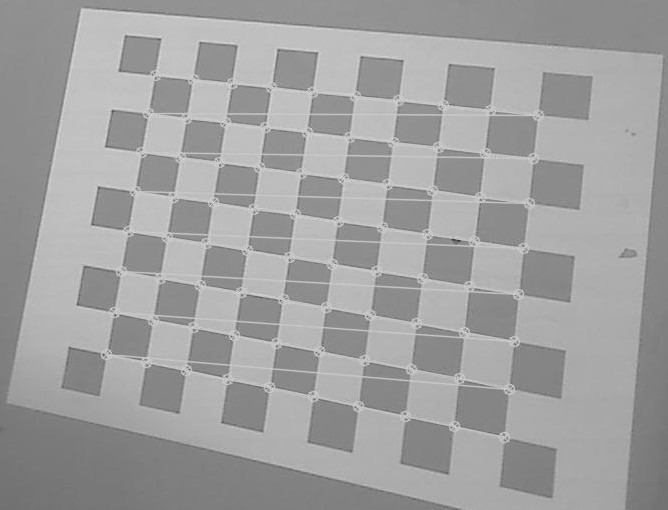
\includegraphics[width=3cm,height=3cm]{../Thesis_work/Latex_thesis_work/img_source/proj_view_3.png}} &  
\hspace{-0.3cm}\subfloat[]{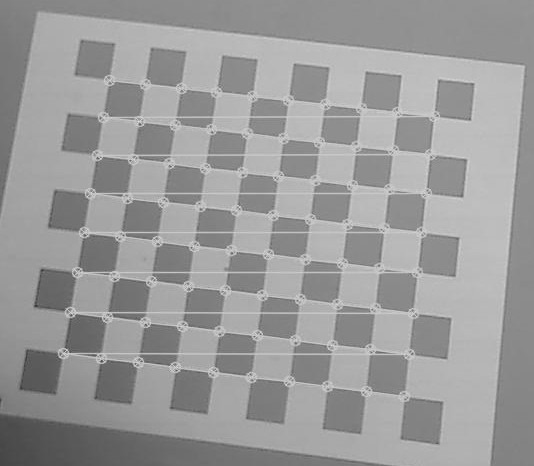
\includegraphics[width=3cm,height=3cm]{../Thesis_work/Latex_thesis_work/img_source/proj_view_4.png}} \\  
\end{tabular}  
\end{tabularx}  
\caption{Some view used for projector calibration} 
\label{fig:proj_calib_view} 
\end{figure} 
\vspace{-0.6cm}
\begin{table}[h]  
\centering  
\begin{tabular}{c l}  
\hline\noalign{\smallskip}  
Parameter & Estimated value \\  
\noalign{\smallskip}\hline\noalign{\smallskip}  
$f_x$ & 2261.710\\  
$f_y$ & 2262.799\\  
$c_x$ & 522.666\\  
$c_y$ & 713.840\\  
\noalign{\smallskip}\hline  
\end{tabular}  
\caption{Estimated Projector intrinsic model parameters}  
\end{table}  
\end{frame}
%%%%%%%%%%%%%%%%%%%%%%%%%%%%%%%%%%%%%%%%%%%%%%%%%%%%%%%%%%%%%%%%%%%%%%%%%%%%SLIDE ENDS%%%%%%%%%%%%%%%%%%%%%%%%%%%%%%%%%%%%%%%


%%%%%%%%%%%%%%%%%%%%%%%%%%%%%%%%%%%%%%%%%%%%%%%%%%%%%%%%%%%%%%%%%%%%%%%%%%%%%SLIDE starts%%%%%%%%%%%%%%%%%%%%%%%%%%%%%%%%%%%%%
\begin{frame}
\begin{figure} 
\begin{tabularx}{\linewidth}{@{}cXX@{}}
\begin{tabular}{l r}
\hspace{-0.3cm}\subfloat[View along X-axis]{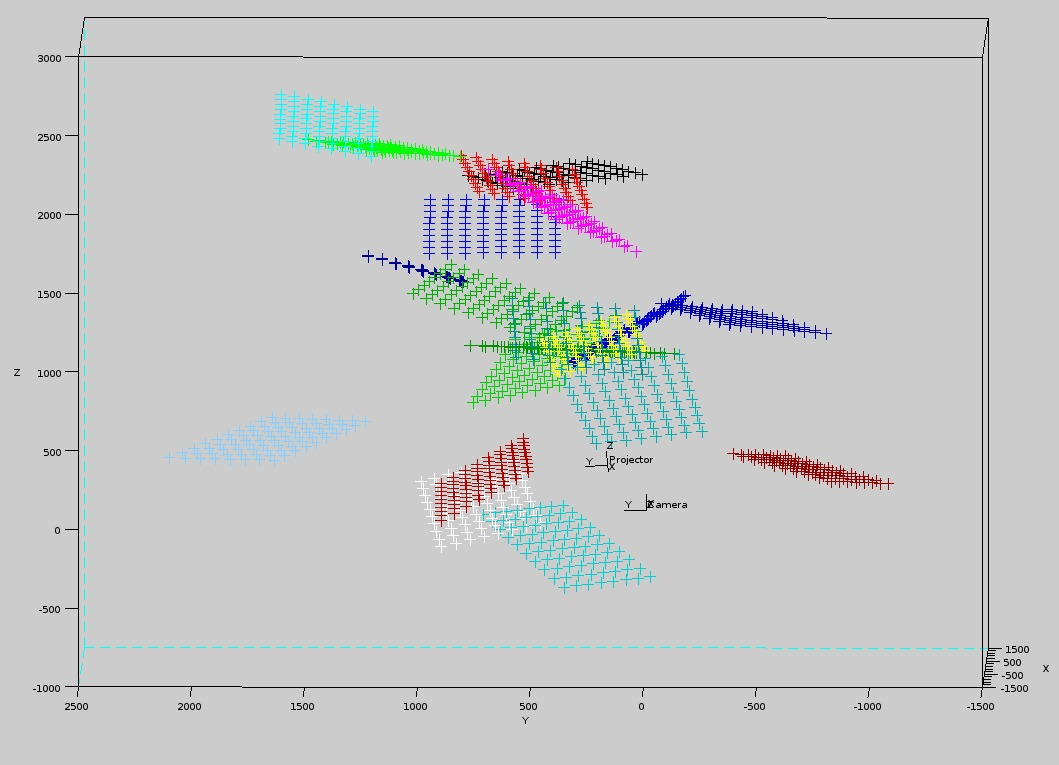
\includegraphics[width=6cm,height=6cm]{../Thesis_work/Latex_thesis_work/img_source/proj_calib_plot_2.png}} &
\subfloat[View along Y-axis]{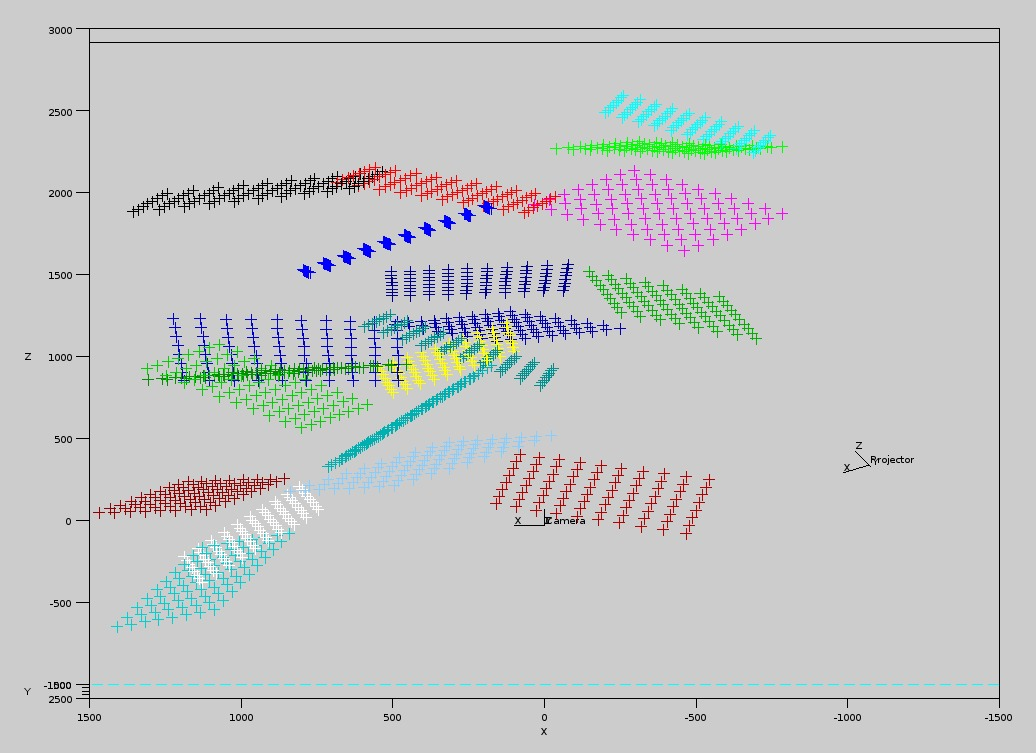
\includegraphics[width=6cm,height=6cm]{../Thesis_work/Latex_thesis_work/img_source/proj_calib_plot_1.png}} \\  
\end{tabular}
\end{tabularx} 
\caption{Visualization of projector calibration results} 
\end{figure}  
\end{frame}
%%%%%%%%%%%%%%%%%%%%%%%%%%%%%%%%%%%%%%%%%%%%%%%%%%%%%%%%%%%%%%%%%%%%%%%%%%%%SLIDE ENDS%%%%%%%%%%%%%%%%%%%%%%%%%%%%%%%%%%%%%%%

%%%%%%%%%%%%%%%%%%%%%%%%%%%%%%%%%%%%%%%%%%%%%%%%%%%%%%%%%%%%%%%%%%%%%%%%%%%%%SLIDE starts%%%%%%%%%%%%%%%%%%%%%%%%%%%%%%%%%%%%%
\begin{frame}
\frametitle{Projector-camera extrinsic calibration}
Estimating rotation and translation vectors for transforming a point in projector coordinate system to camera coordinate system.
\begin{equation}  
\begin{bmatrix}  
P_c \\  
P_p  
\end{bmatrix}  
=\begin{bmatrix}  
R_{wc}*P_w \\  
R_{wp}*P_w  
\end{bmatrix}  
+\begin{bmatrix}  
T_{wc} \\  
T_{wp}  
\end{bmatrix}  
\end{equation}  
hence,\newline  
$P_c=\underbrace{(R_c*R_p^{-1})}_{R_{pc}}*P_p+\underbrace{(T_c-R_c*R_p^{-1}*P_p)}_{T_{pc}}$  
\vspace{-0.5cm}
\begin{figure}
\begin{tabularx}{\linewidth}{@{}cXX@{}}  
\begin{tabular}{c c}
\subfloat[]{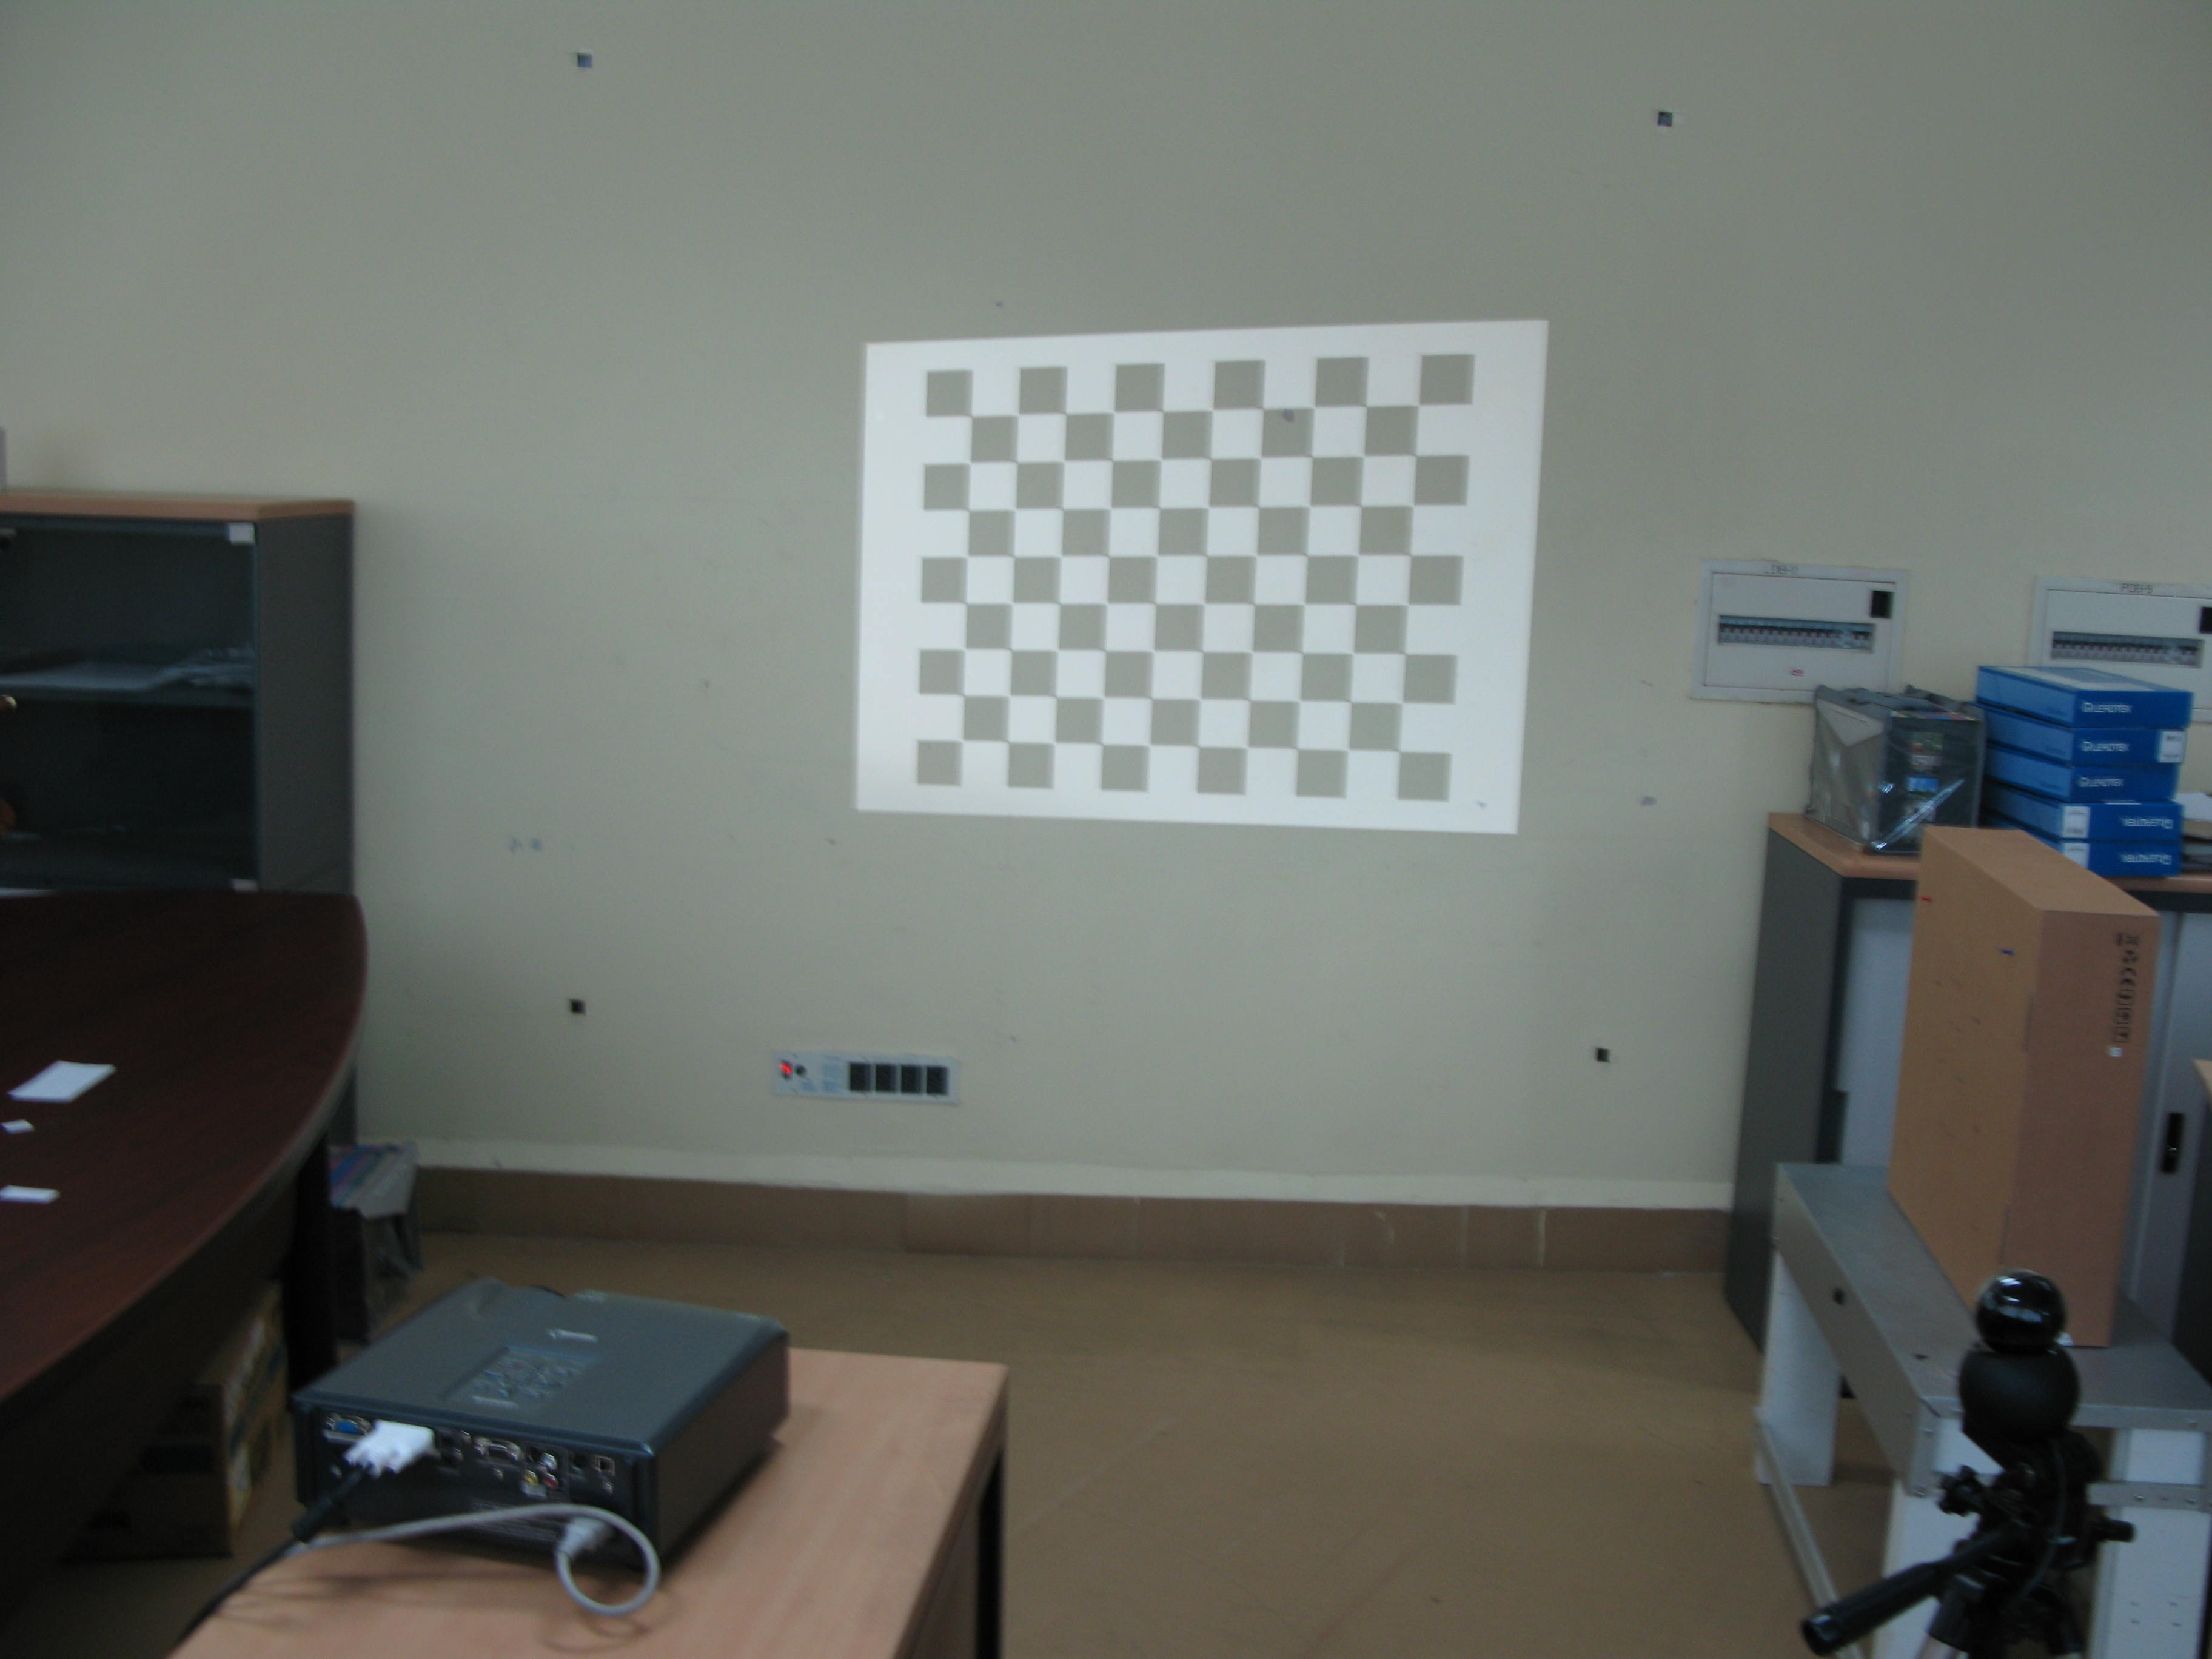
\includegraphics[width=5cm,height=5cm]{../Thesis_work/Latex_thesis_work/img_source/system_extrinsic.png}}  
\subfloat[]{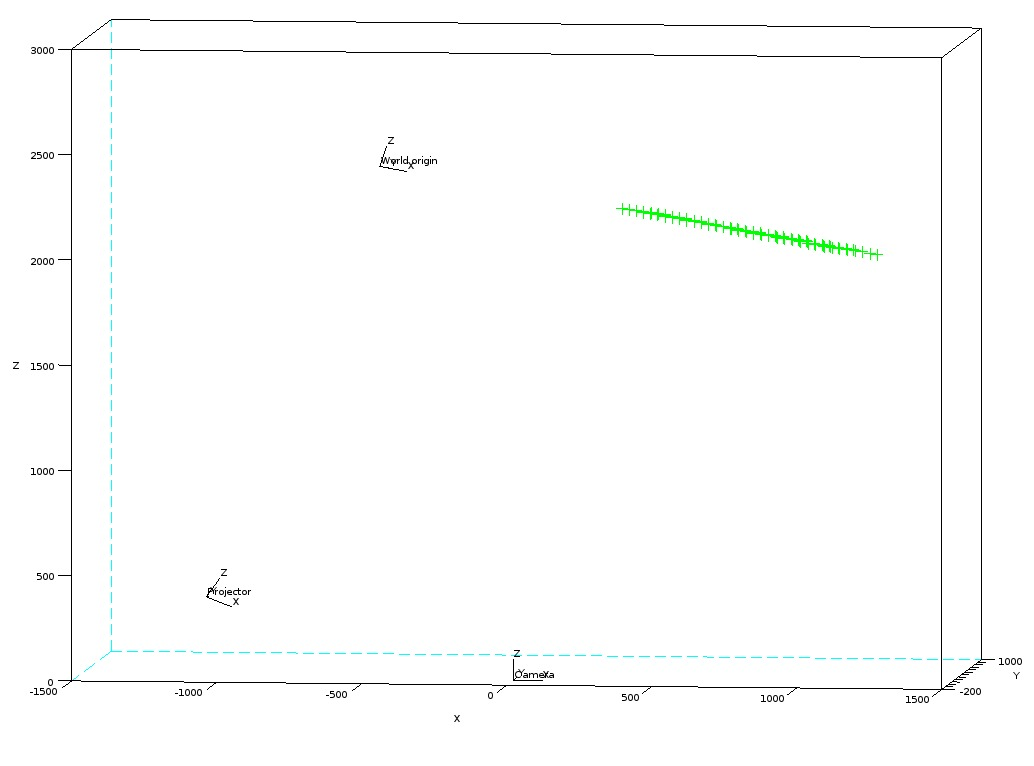
\includegraphics[width=7cm,height=5cm]{../Thesis_work/Latex_thesis_work/img_source/system_plot.png}}
\end{tabular}
\end{tabularx}
\label{fig:extrinsic_calib_setup}
\end{figure}  
\end{frame}
%%%%%%%%%%%%%%%%%%%%%%%%%%%%%%%%%%%%%%%%%%%%%%%%%%%%%%%%%%%%%%%%%%%%%%%%%%%%SLIDE ENDS%%%%%%%%%%%%%%%%%%%%%%%%%%%%%%%%%%%%%%%


%%%%%%%%%%%%%%%%%%%%%%%%%%%%%%%%%%%%%%%%%%%%%%%%%%%%%%%%%%%%%%%%%%%%%%%%%%%%%SLIDE starts%%%%%%%%%%%%%%%%%%%%%%%%%%%%%%%%%%%%%
\begin{frame}
\frametitle{Triangulation module}
To assign 3D coordinates to a point viewed by both camera and projector,\newline
For camera,
\begin{equation}
\begin{bmatrix}
w_c*u_i^c \\
w_c*v_i^c \\
w_c
\end{bmatrix}
=\begin{bmatrix}
a_{1,1}^c & a_{1,2}^c & a_{1,3}^c & a_{1,4}^c \\
a_{2,1}^c & a_{2,2}^c & a_{2,3}^c & a_{2,4}^c \\
a_{3,1}^c & a_{3,2}^c & a_{3,3}^c & a_{3,4}^c 
\end{bmatrix}
\begin{bmatrix}
x_i^w\\
y_i^w\\
z_i^w\\
1
\end{bmatrix}
\end{equation}
Similarly,for projector,
\begin{equation}
\begin{bmatrix}
w_c*u_i^p \\
w_c*v_i^p \\
w_p
\end{bmatrix}
=\begin{bmatrix}
a_{1,1}^p & a_{1,2}^p & a_{1,3}^p & a_{1,4}^p \\
a_{2,1}^p & a_{2,2}^p & a_{2,3}^p & a_{2,4}^p \\
a_{3,1}^p & a_{3,2}^p & a_{3,3}^p & a_{3,4}^p 
\end{bmatrix}
\begin{bmatrix}
x_i^w\\
y_i^w\\
z_i^w\\
1
\end{bmatrix}
\end{equation}
In matrix form it can be written as,
\begin{equation}
PV=F
\end{equation}
\noindent
where,\newline
\newline
P=$\begin{bmatrix}
(a_{1,1}^c-u_i^ca_{3,1}^c) & (a_{1,2}^c-u_i^ca_{3,2}^c) & (a_{1,3}^c-u_i^ca_{3,3}^c) \\ (a_{2,1}^c-v_i^ca_{3,1}^c) & (a_{2,2}^c-v_i^ca_{3,2}^c) & (a_{2,3}^c-v_i^ca_{3,3}^c) \\
(a_{1,1}^p-u_i^pa_{3,1}^p) & (a_{1,2}^p-u_i^pa_{3,2}^p) & (a_{1,3}^p-u_i^pa_{3,3}^p) \\ (a_{2,1}^p-v_i^pa_{3,1}^p) & (a_{2,2}^p-v_i^pa_{3,2}^p) & (a_{2,3}^p-v_i^pa_{3,3}^p)
\end{bmatrix},V=\begin{bmatrix}
x_i^w\\
y_i^w\\
z_i^w
\end{bmatrix},F=\begin{bmatrix}
a_{3,4}^cu_i^c-a_{1,4}^c\\
a_{3,4}^cv_i^c-a_{2,4}^c\\
a_{3,4}^pu_i^p-a_{1,4}^p\\
a_{3,4}^pv_i^p-a_{2,4}^p
\end{bmatrix}$\newline 
\end{frame}
%%%%%%%%%%%%%%%%%%%%%%%%%%%%%%%%%%%%%%%%%%%%%%%%%%%%%%%%%%%%%%%%%%%%%%%%%%%%SLIDE ENDS%%%%%%%%%%%%%%%%%%%%%%%%%%%%%%%%%%%%%%%

%%%%%%%%%%%%%%%%%%%%%%%%%%%%%%%%%%%%%%%%%%%%%%%%%%%%%%%%%%%%%%%%%%%%%%%%%%%%%SLIDE starts%%%%%%%%%%%%%%%%%%%%%%%%%%%%%%%%%%%%%
\begin{frame}
Results of applying equation $PV=F$,
\begin{figure}
%\def\tabularxcolumn#1{m{#1}}
\begin{tabularx}{\linewidth}{@{}cXX@{}}
\begin{tabular}{c c c c}
\hspace{-0.3cm}\subfloat[2D face image]{\includegraphics[width=3cm,height=3cm]{../Thesis_work/Latex_thesis_work/img_source/face_2d.png}} & 
\hspace{-0.3cm}\subfloat[3D reconstruction of face]{\includegraphics[width=3cm,height=3cm]{../Thesis_work/Latex_thesis_work/img_source/face_3d.png}} &
\hspace{-0.3cm}\subfloat[2D image of box in front of wall]{\includegraphics[width=3cm,height=3cm]{../Thesis_work/Latex_thesis_work/img_source/box_wall_2d.png}} & 
\hspace{-0.3cm}\subfloat[3D reconstruction of box in front of wall]{\includegraphics[width=3cm,height=3cm]{../Thesis_work/Latex_thesis_work/img_source/box_wall_3d.png}}\\
\hspace{-0.3cm}\subfloat[2D image of a chair with background]{\includegraphics[width=3cm,height=3cm]{../Thesis_work/Latex_thesis_work/img_source/chair_2d.png}} &
\hspace{-0.3cm}\subfloat[3D reconstruction of chair with background]{\includegraphics[width=3cm,height=3cm]{../Thesis_work/Latex_thesis_work/img_source/chair_reconstruction.png}} &
\hspace{-0.3cm}\subfloat[A cup]{\includegraphics[width=3cm,height=3cm]{../Thesis_work/Latex_thesis_work/img_source/cup_2d.png}} &
\hspace{-0.3cm}\subfloat[3D reconstruction of cup]{\includegraphics[width=3cm,height=3cm]{../Thesis_work/Latex_thesis_work/img_source/cup_3d.png}}\\ 
\end{tabular}
\end{tabularx}
\caption{Some 3D reconstruction results}
\end{figure}
\end{frame}
%%%%%%%%%%%%%%%%%%%%%%%%%%%%%%%%%%%%%%%%%%%%%%%%%%%%%%%%%%%%%%%%%%%%%%%%%%%%SLIDE ENDS%%%%%%%%%%%%%%%%%%%%%%%%%%%%%%%%%%%%%%%

\end{document} 
